\documentclass[a4paper]{article}
\usepackage{pdfpages}
\usepackage[magyar]{babel}
\usepackage[T1]{fontenc}
\usepackage[utf8]{inputenc}

\usepackage{geometry}

\geometry{
    bmargin=2cm
}

\usepackage[tocflat]{tocstyle}
\usetocstyle{standard}

\usepackage[linktocpage]{hyperref}

\begin{document}

\begin{titlepage}

    \centering
    
\includegraphics[width=0.66\textwidth]{elte.jpg}\par\vspace{1cm}
    {\scshape\LARGE Eötvös Loránd University \par}
    \vspace{1cm}
    \rule{140mm}{0.1mm}\\
    \vspace{.5cm}
    {\scshape\Large Scientific Data Analytics and Modeling \\ specialization \par}
    \vspace{.5cm}
    \rule{140mm}{0.1mm}\\

    \vfill
    
    {\large 2020 \par}
\end{titlepage}

\newpage

\tableofcontents

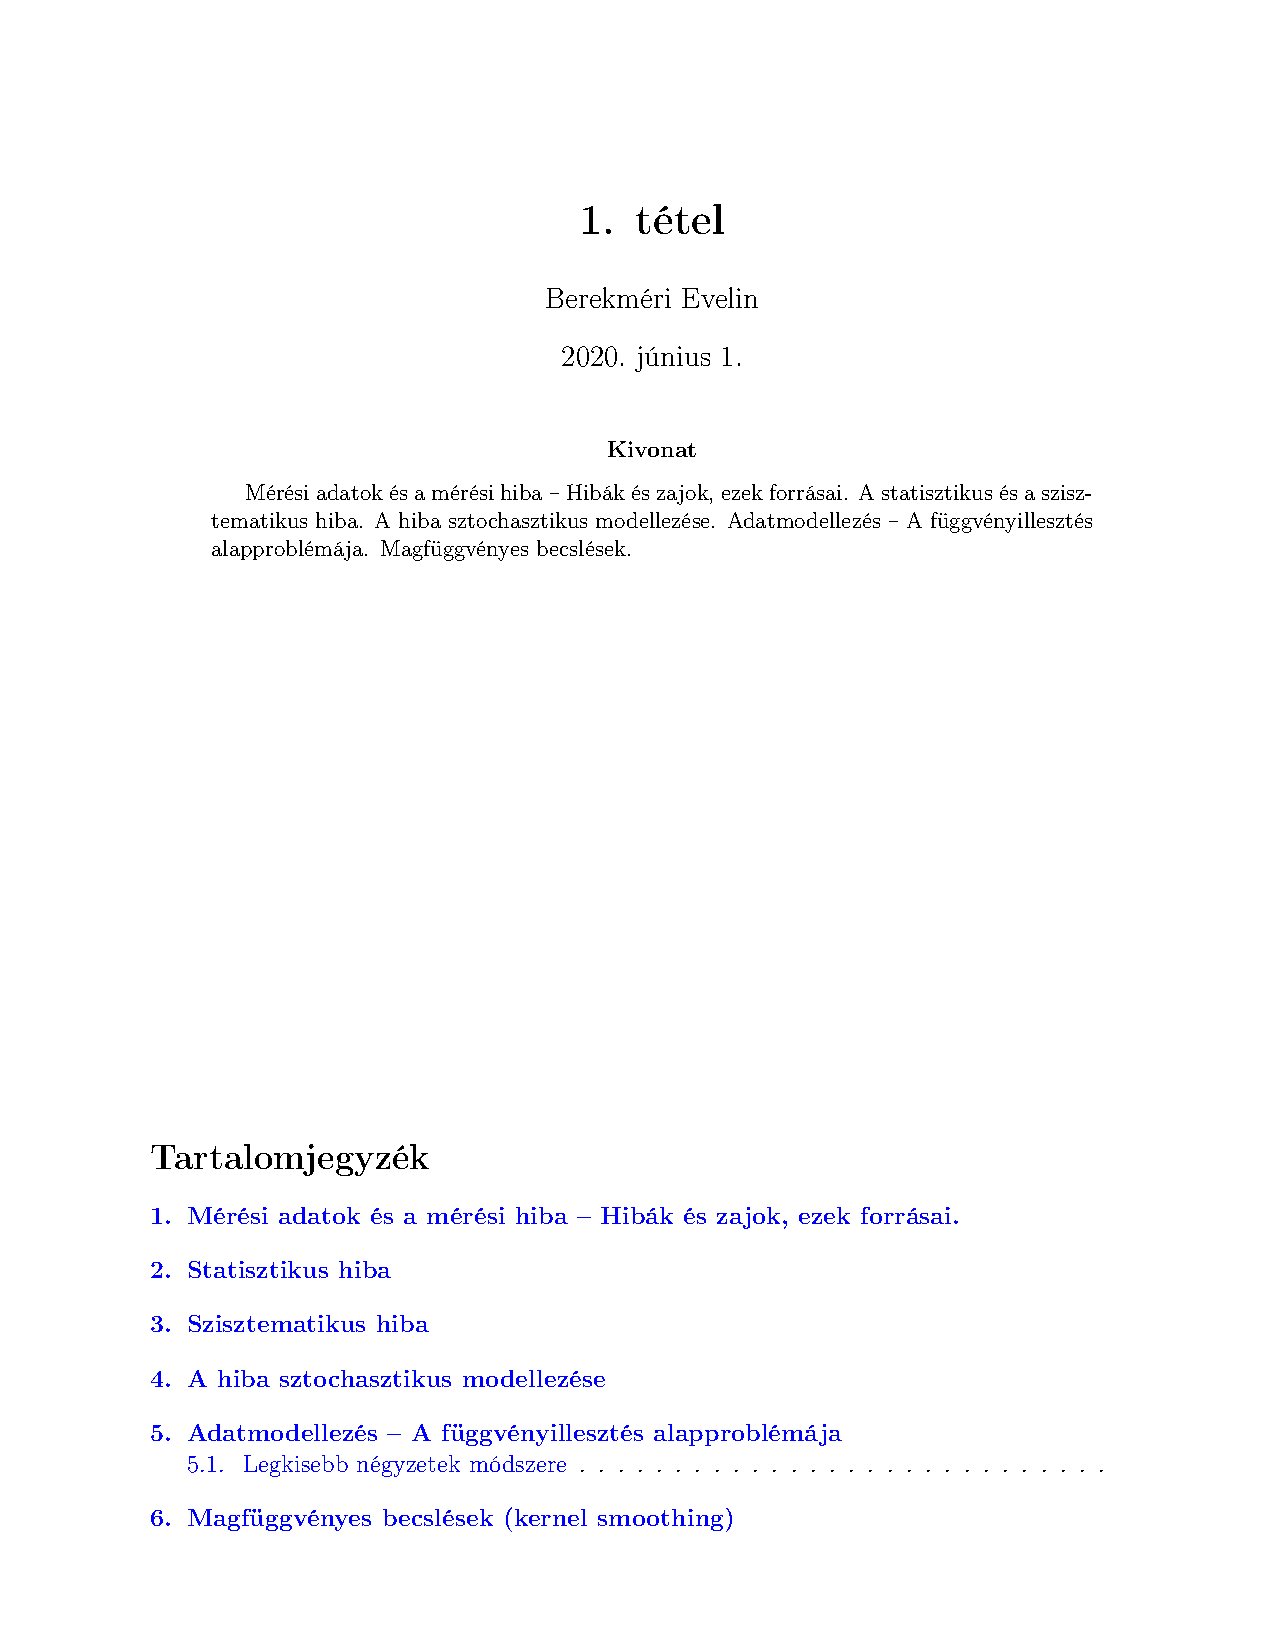
\includepdf[pages=-,addtotoc={
    1,section,1,\textbf{Mérési adatok és a mérési hiba – Hibák és zajok, ezek forrásai. A statisztikus és a szisztematikus hiba. A hiba sztochasztikus modellezése. Adatmodellezés – A függvényillesztés alapproblémája. Magfüggvényes becslések.},p1}, pagecommand={\thispagestyle{plain}}]{../001/1.pdf}

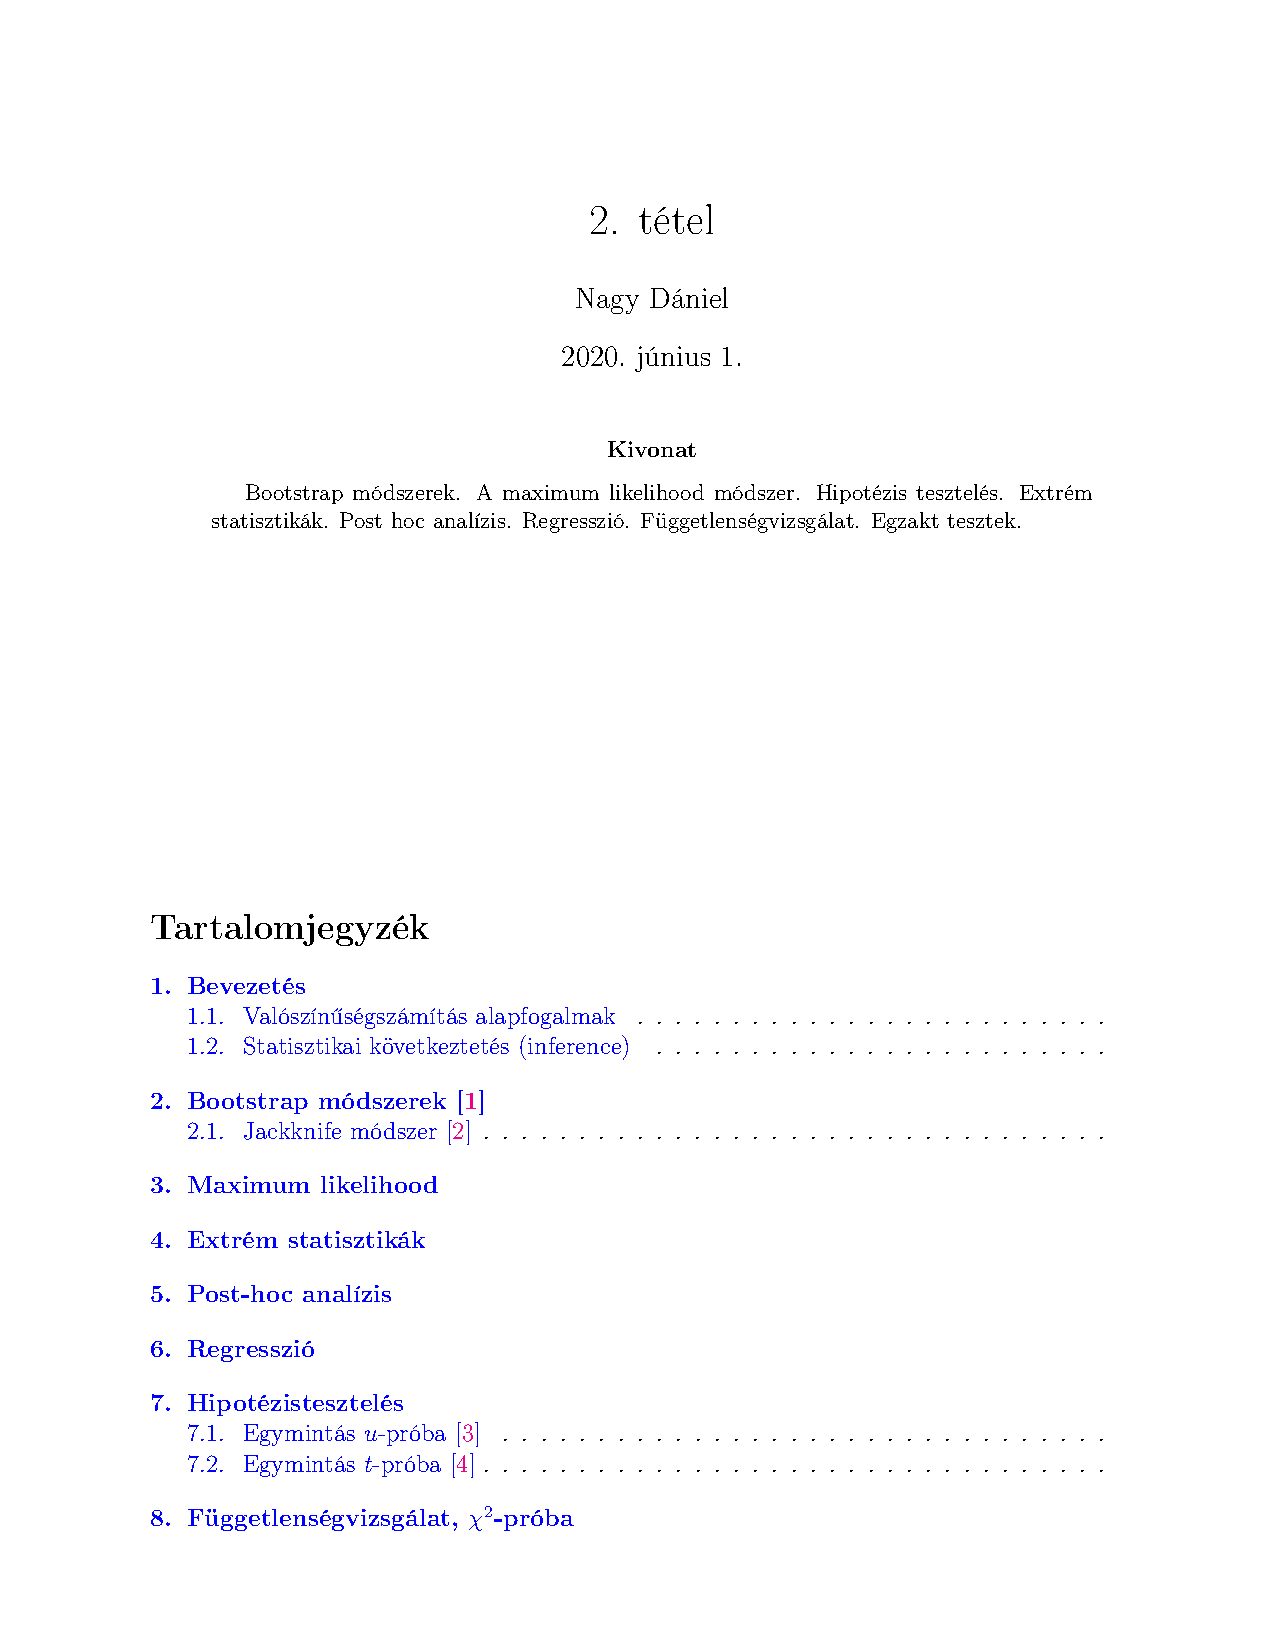
\includepdf[pages=-,addtotoc={
    1,section,1,\textbf{Bootstrap módszerek. A maximum likelihood módszer. Hipotézis tesztelés. Extrém statisztikák. Post hoc analízis. Regresszió. Függetlenségvizsgálat. Egzakt tesztek.},p1}, pagecommand={\thispagestyle{plain}}]{../002/2.pdf}

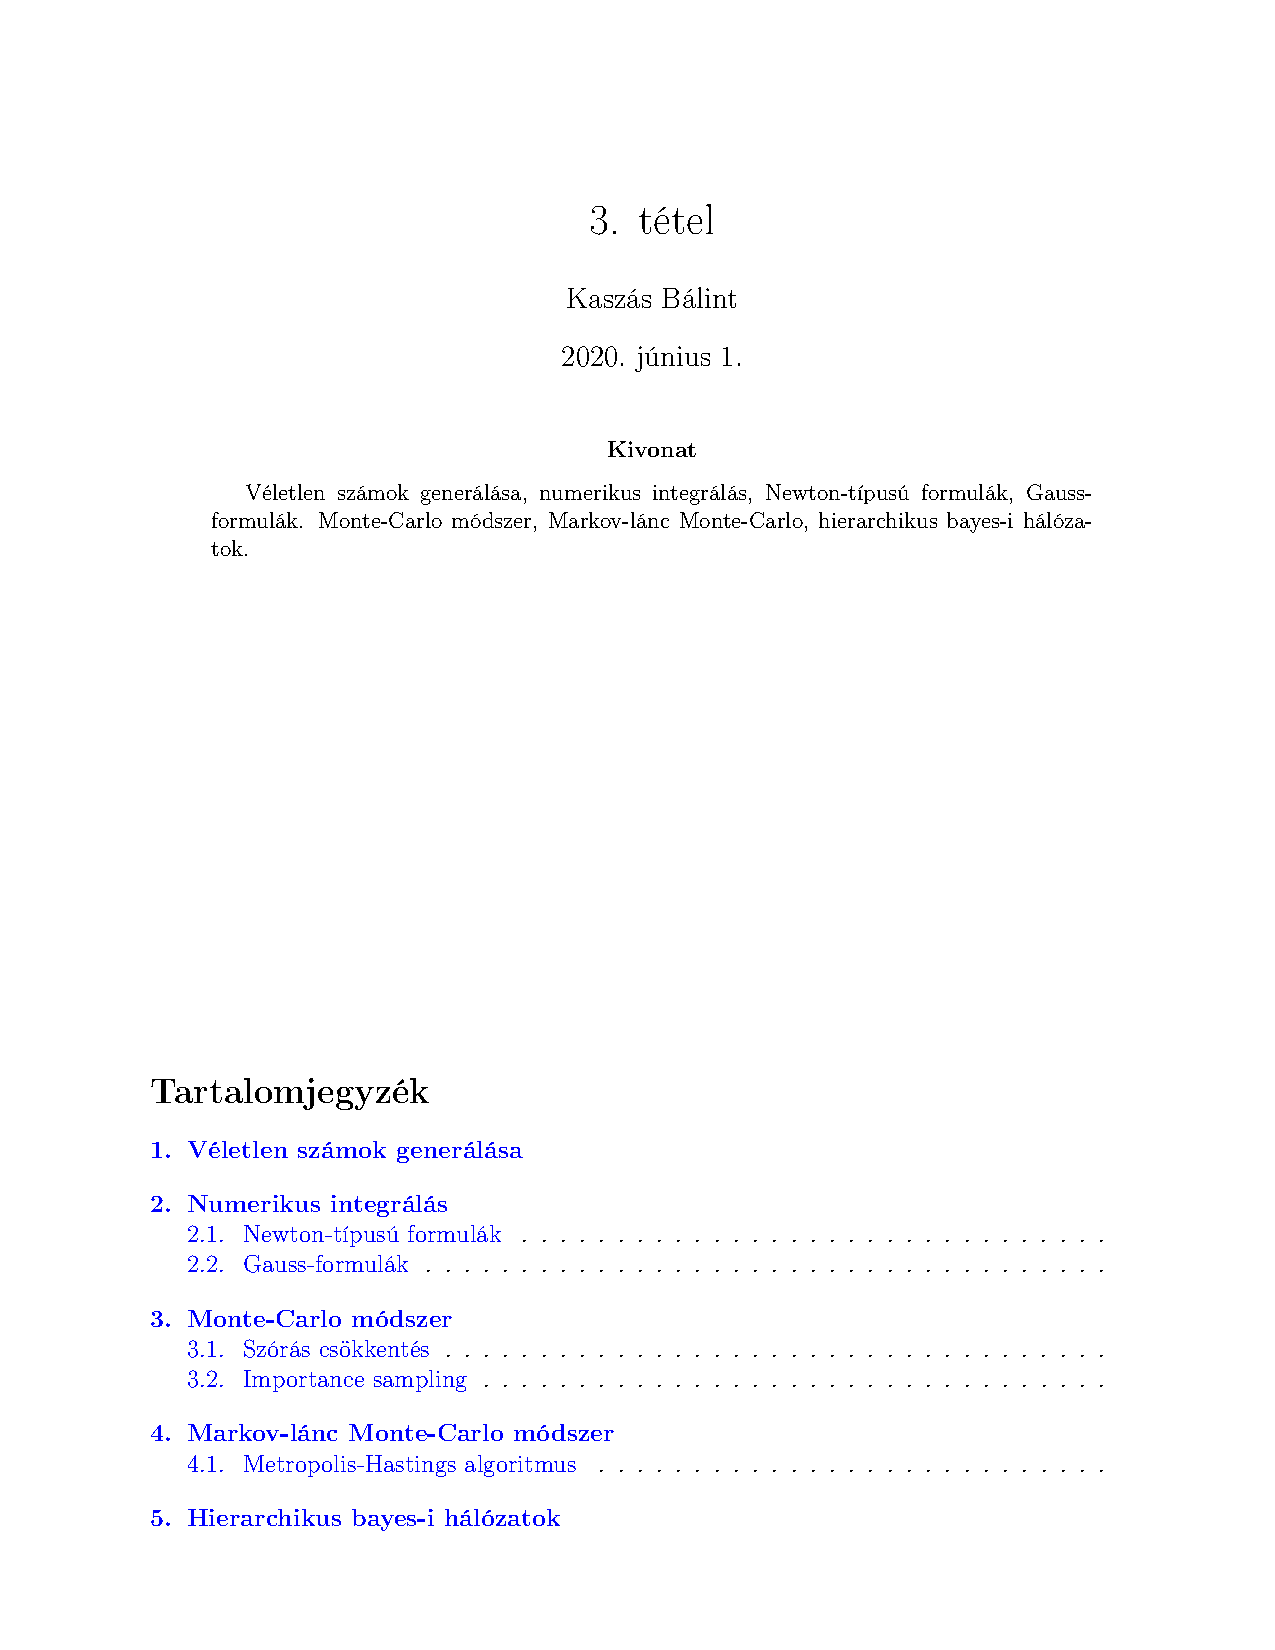
\includepdf[pages=-,addtotoc={
    1,section,1,\textbf{Véletlen számok generálása, numerikus integrálás, Newton-típusú formulák, Gauss-formulák. Monte-Carlo módszer, Markov-lánc Monte-Carlo, hierarchikus bayes-i hálózatok.},p1}, pagecommand={\thispagestyle{plain}}]{../003/3.pdf}

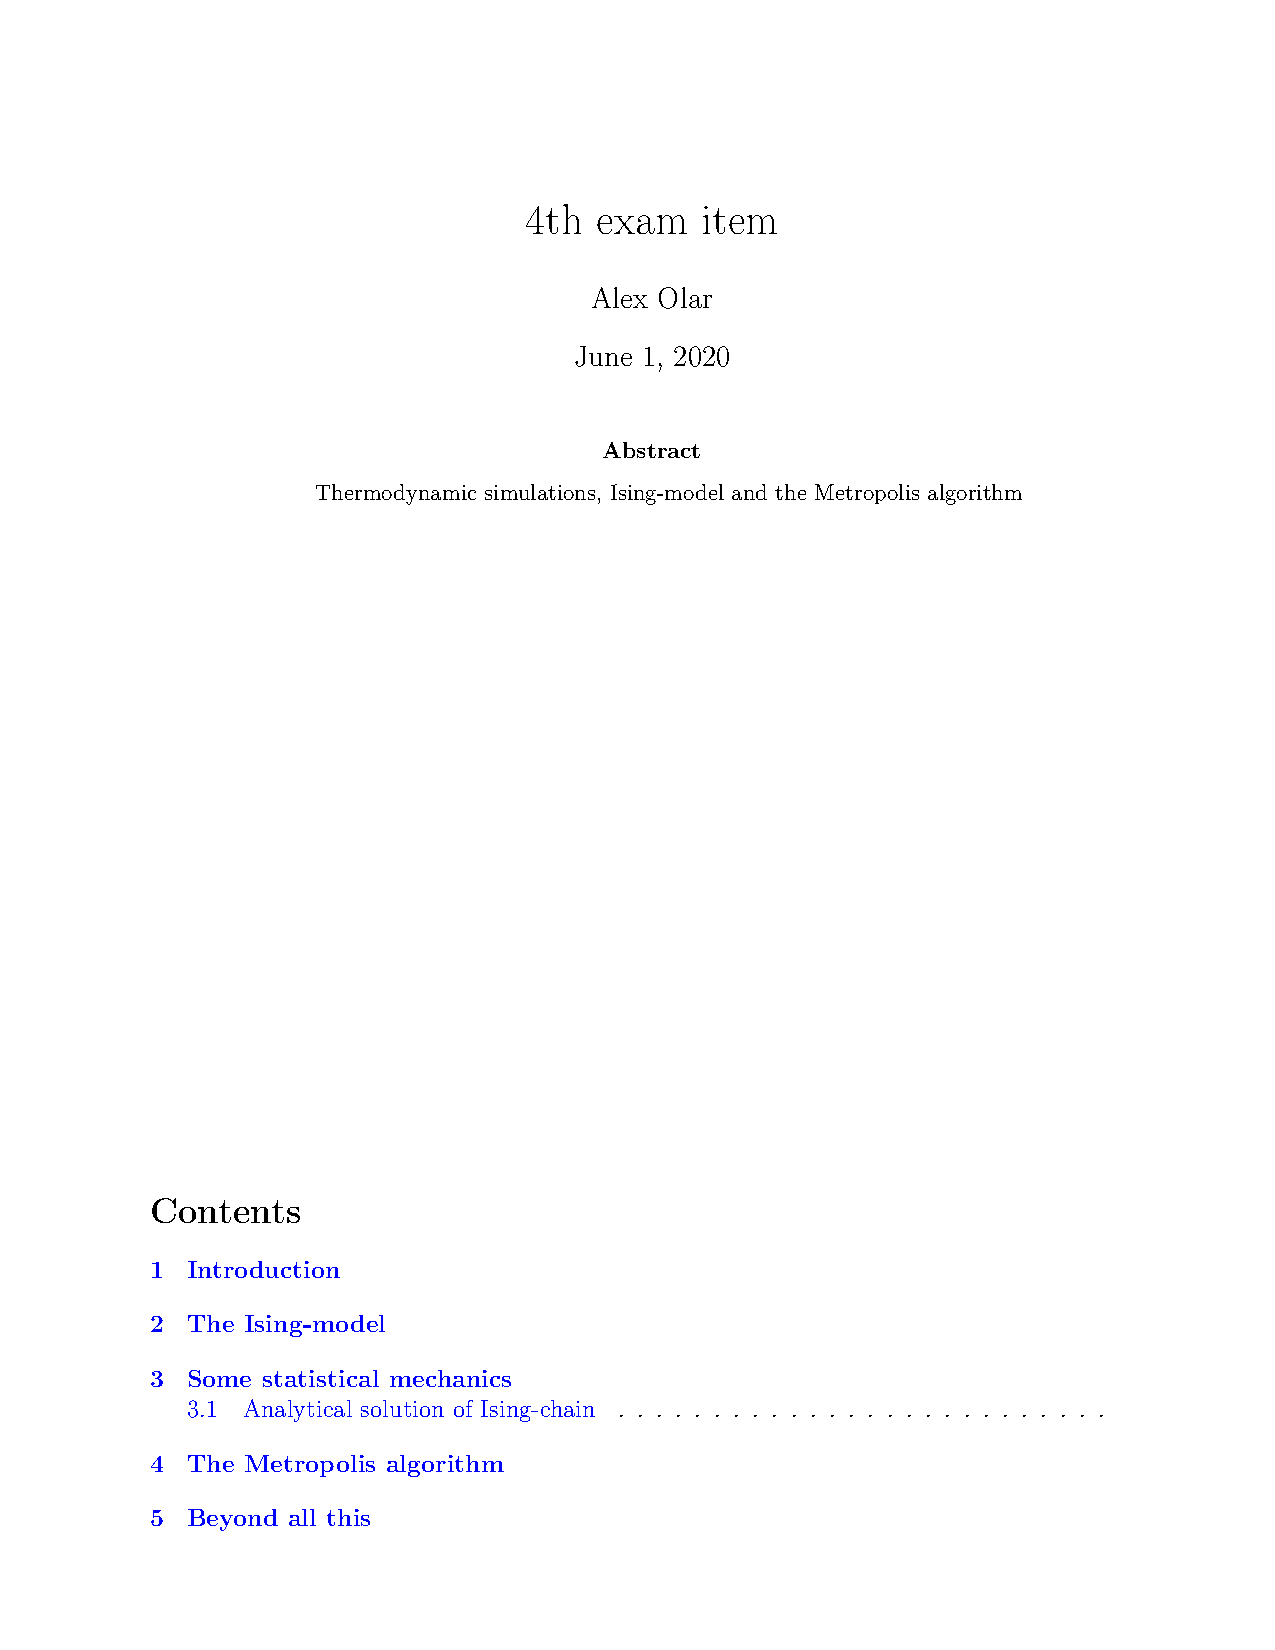
\includepdf[pages=-,addtotoc={
    1,section,1,\textbf{Termodinamikai rendszerek szimulációja, Ising-model, Metropolis-algoritmus.},p1}, pagecommand={\thispagestyle{plain}}]{../004/4.pdf}

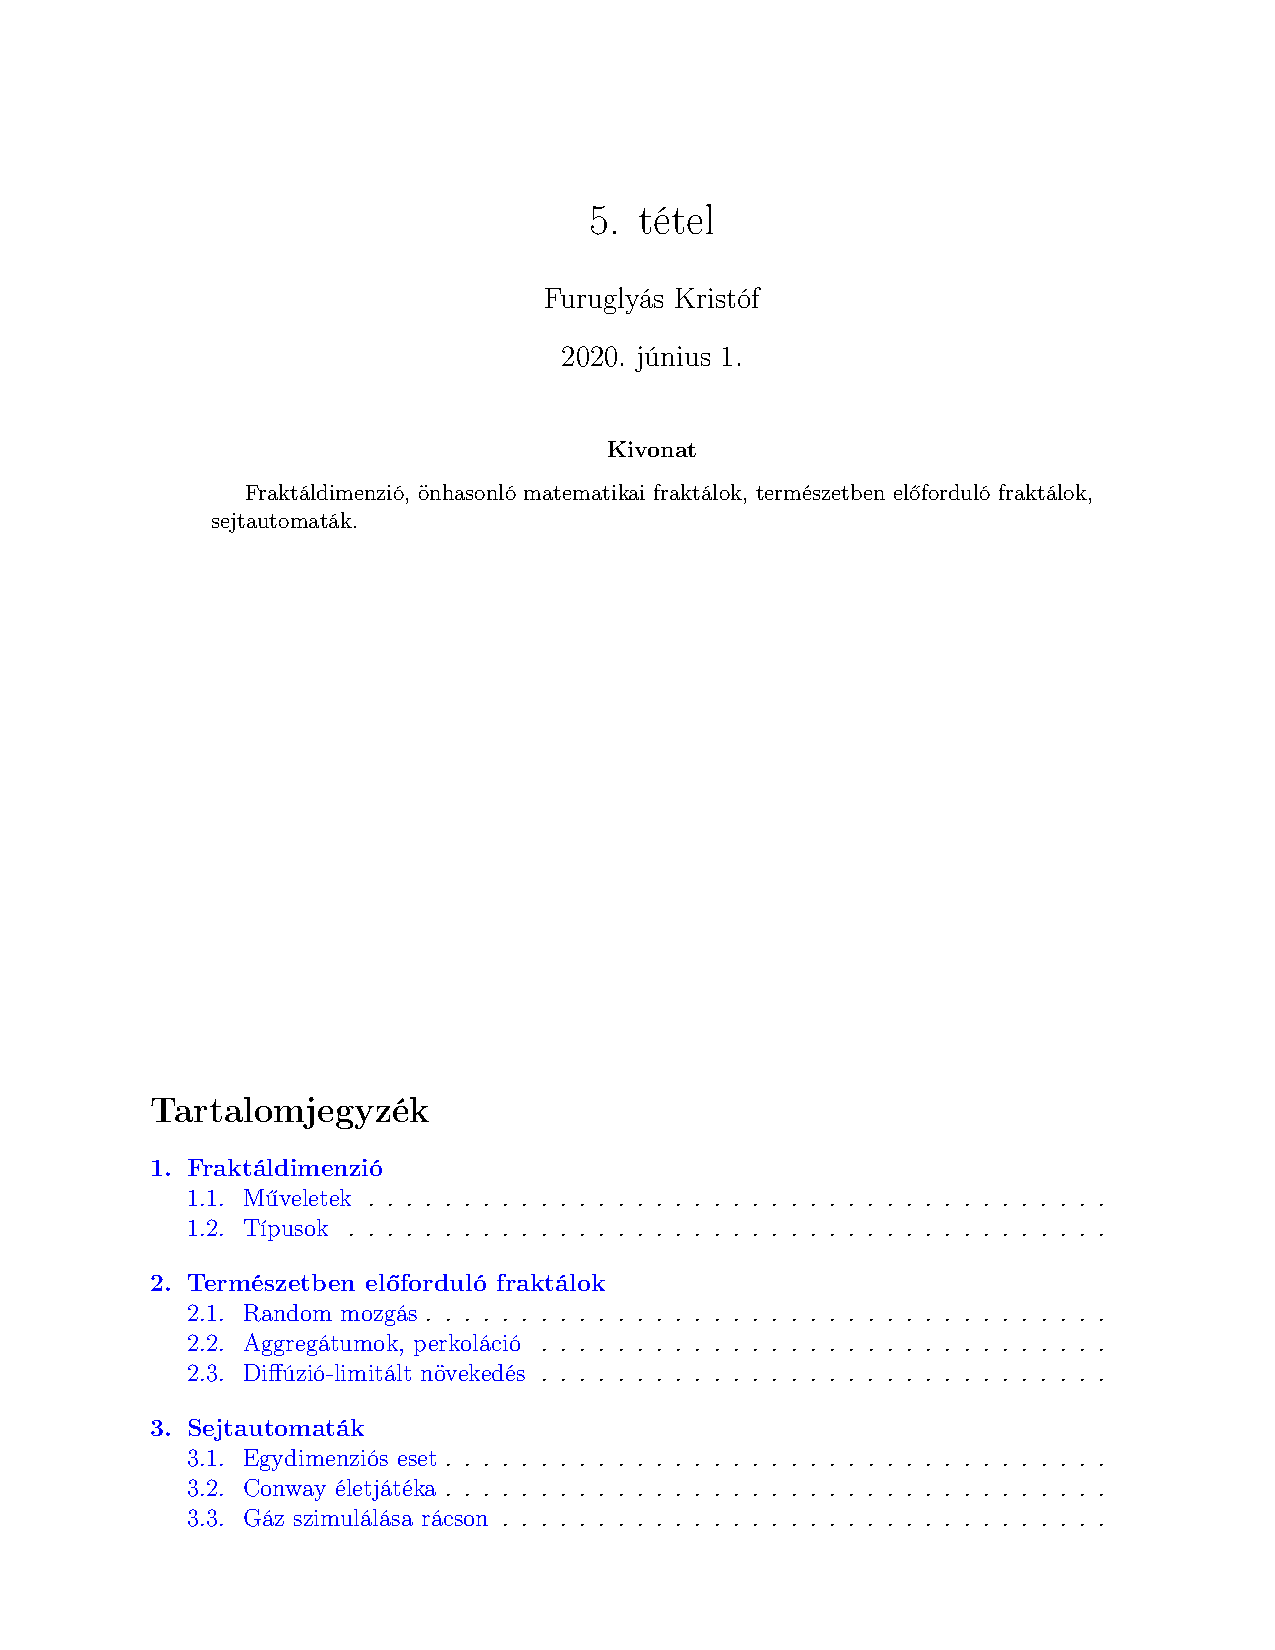
\includepdf[pages=-,addtotoc={
    1,section,1,\textbf{Fraktáldimenzió, önhasonló matematikai fraktálok, természetben előforduló fraktálok, sejtautomaták.},p1}, pagecommand={\thispagestyle{plain}}]{../005/5.pdf}

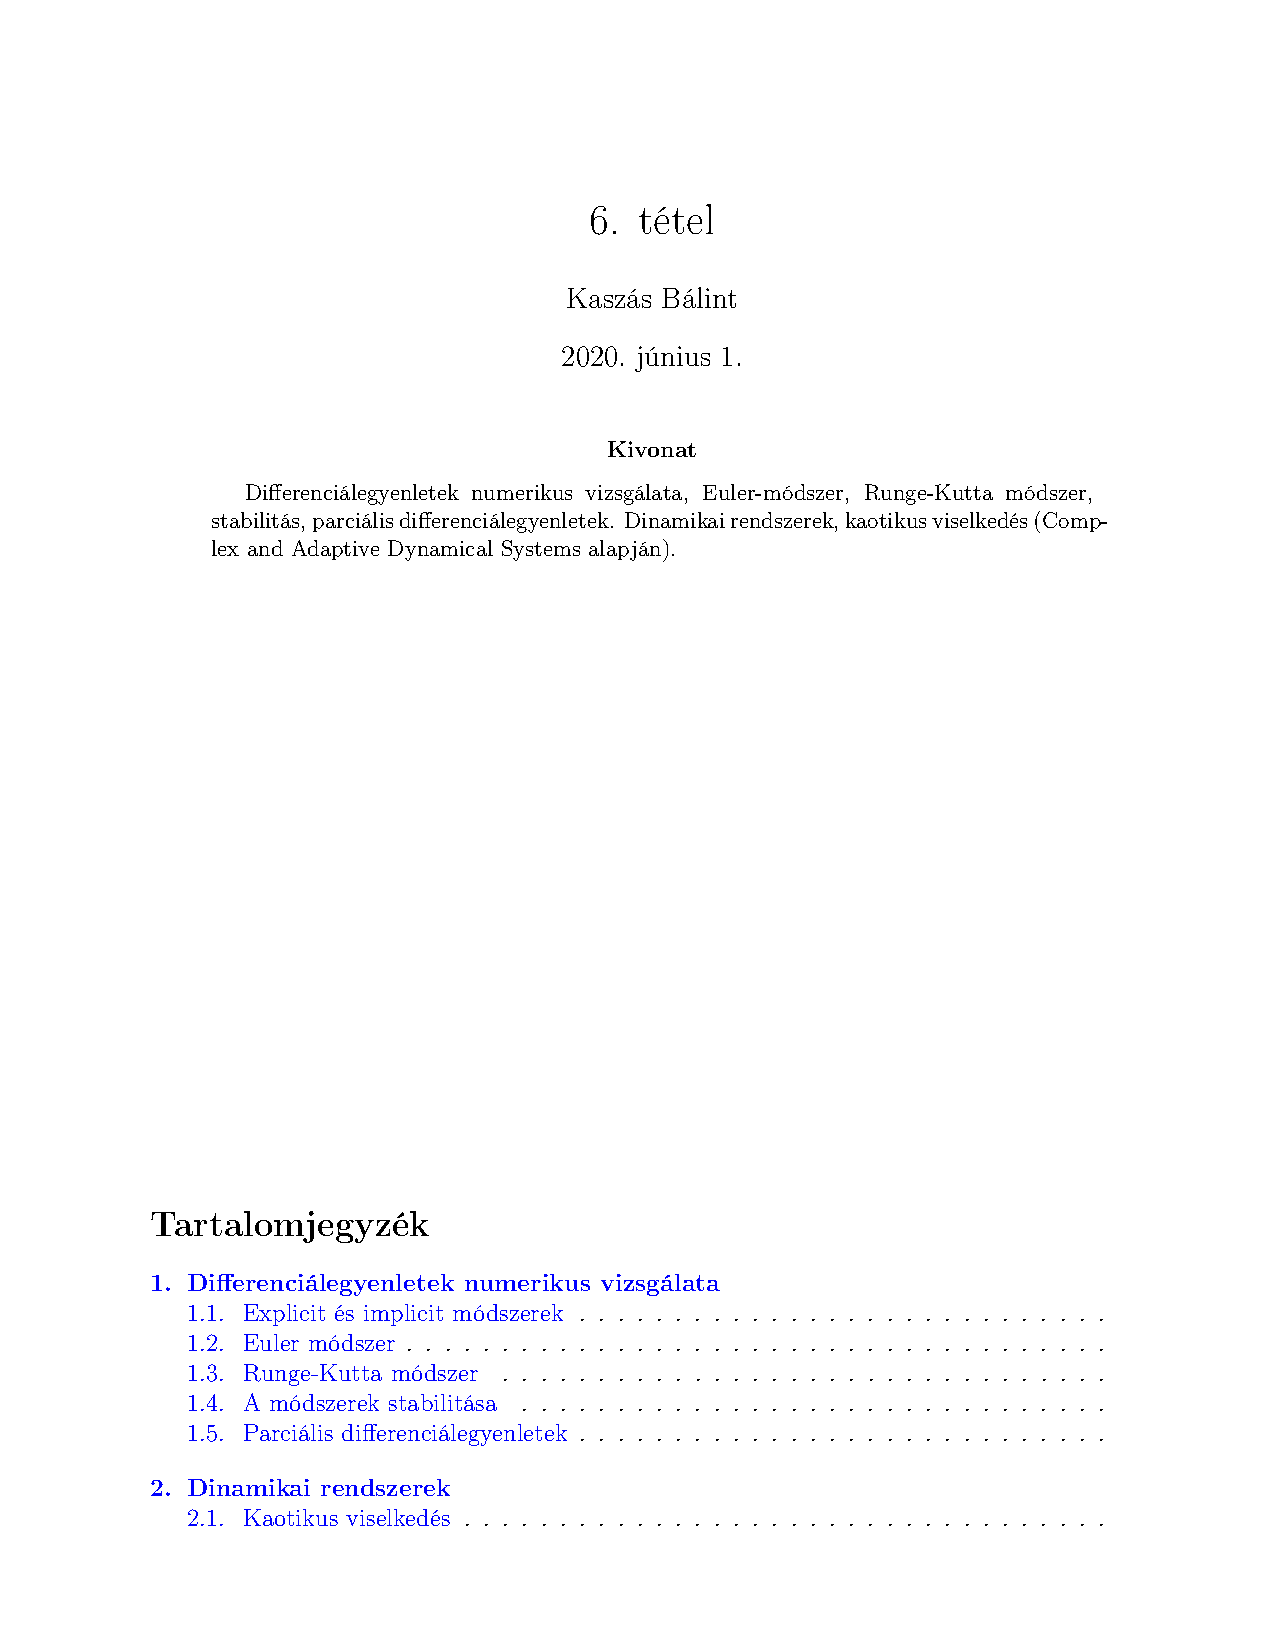
\includepdf[pages=-,addtotoc={
    1,section,1,\textbf{Differenciálegyenletek numerikus vizsgálata, Euler-módszer, Runge-Kutta módszer, stabilitás, parciális differenciálegyenletek. Dinamikai rendszerek, kaotikus viselkedés},p1}, pagecommand={\thispagestyle{plain}}]{../006/6.pdf}

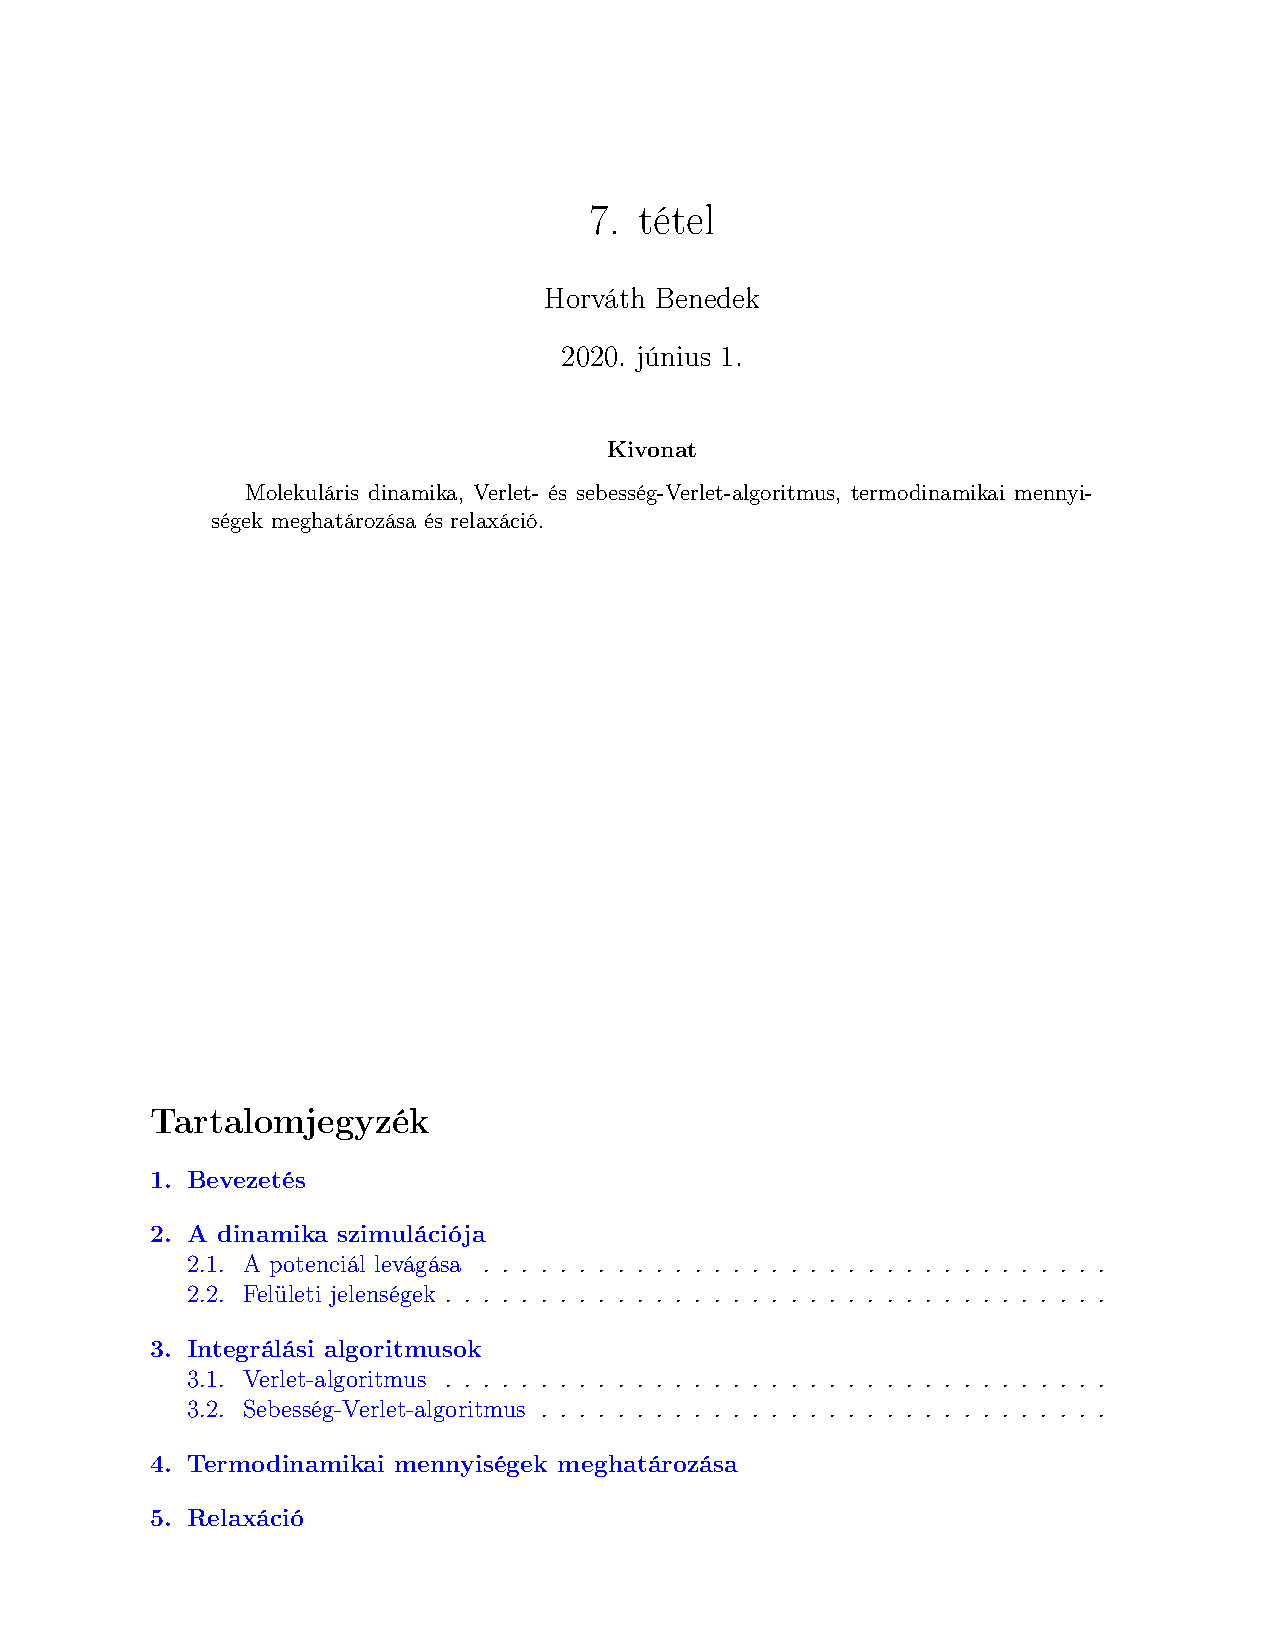
\includepdf[pages=-,addtotoc={
    1,section,1,\textbf{Molekuláris dinamika, Verlet- és sebesség-Verlet-algoritmus, termodinamikai mennyiségek meghatározása és relaxáció.},p1}, pagecommand={\thispagestyle{plain}}]{../007/7.pdf}

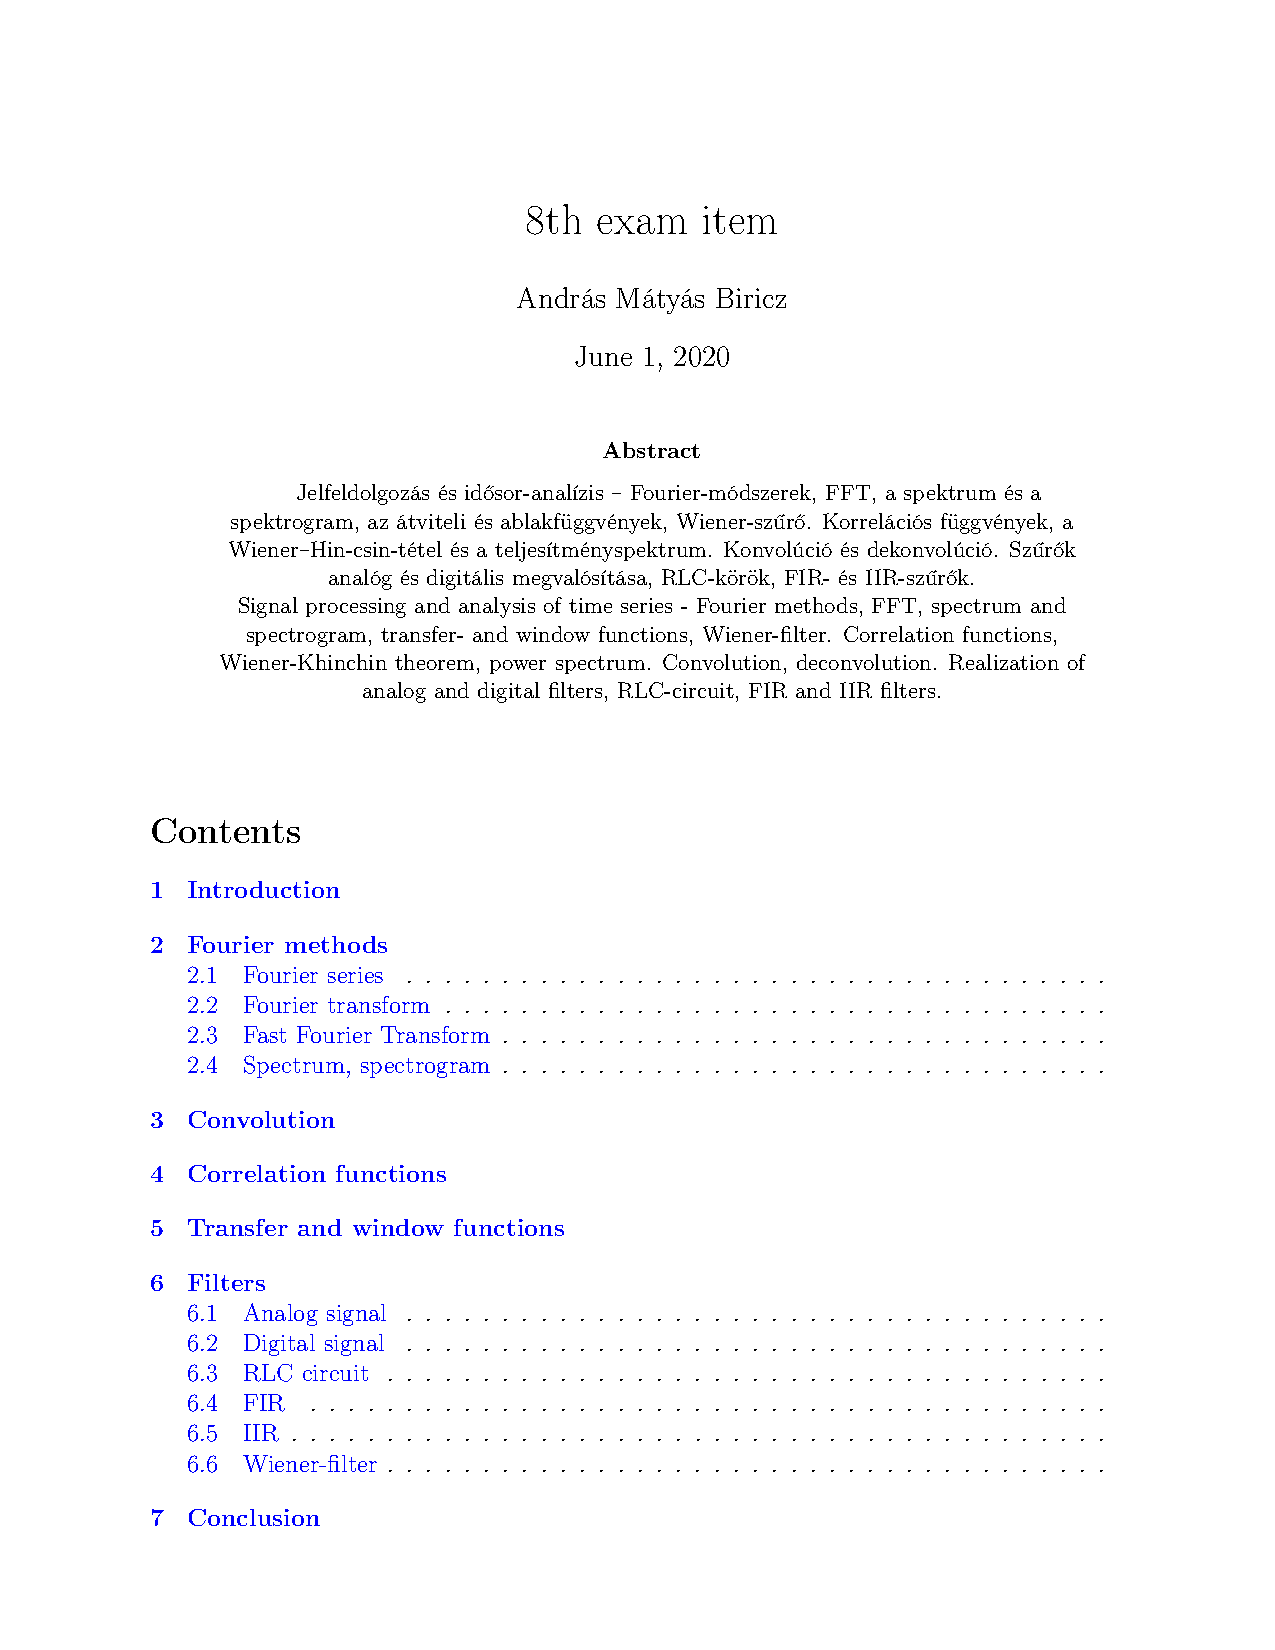
\includepdf[pages=-,addtotoc={
    1,section,1,\textbf{Jelfeldolgozás és idősor-analízis – Fourier-módszerek, FFT, a spektrum és a spektrogram, az átviteli és ablakfüggvények, Wiener-szűrő. Korrelációs függvények, a Wiener–Hincsin-tétel és a teljesítményspektrum. Konvolúció és dekonvolúció. Szűrők analóg és digitális megvalósítása, RLC-körök, FIR- és IIR-szűrők.},p1}, pagecommand={\thispagestyle{plain}}]{../008/8.pdf}

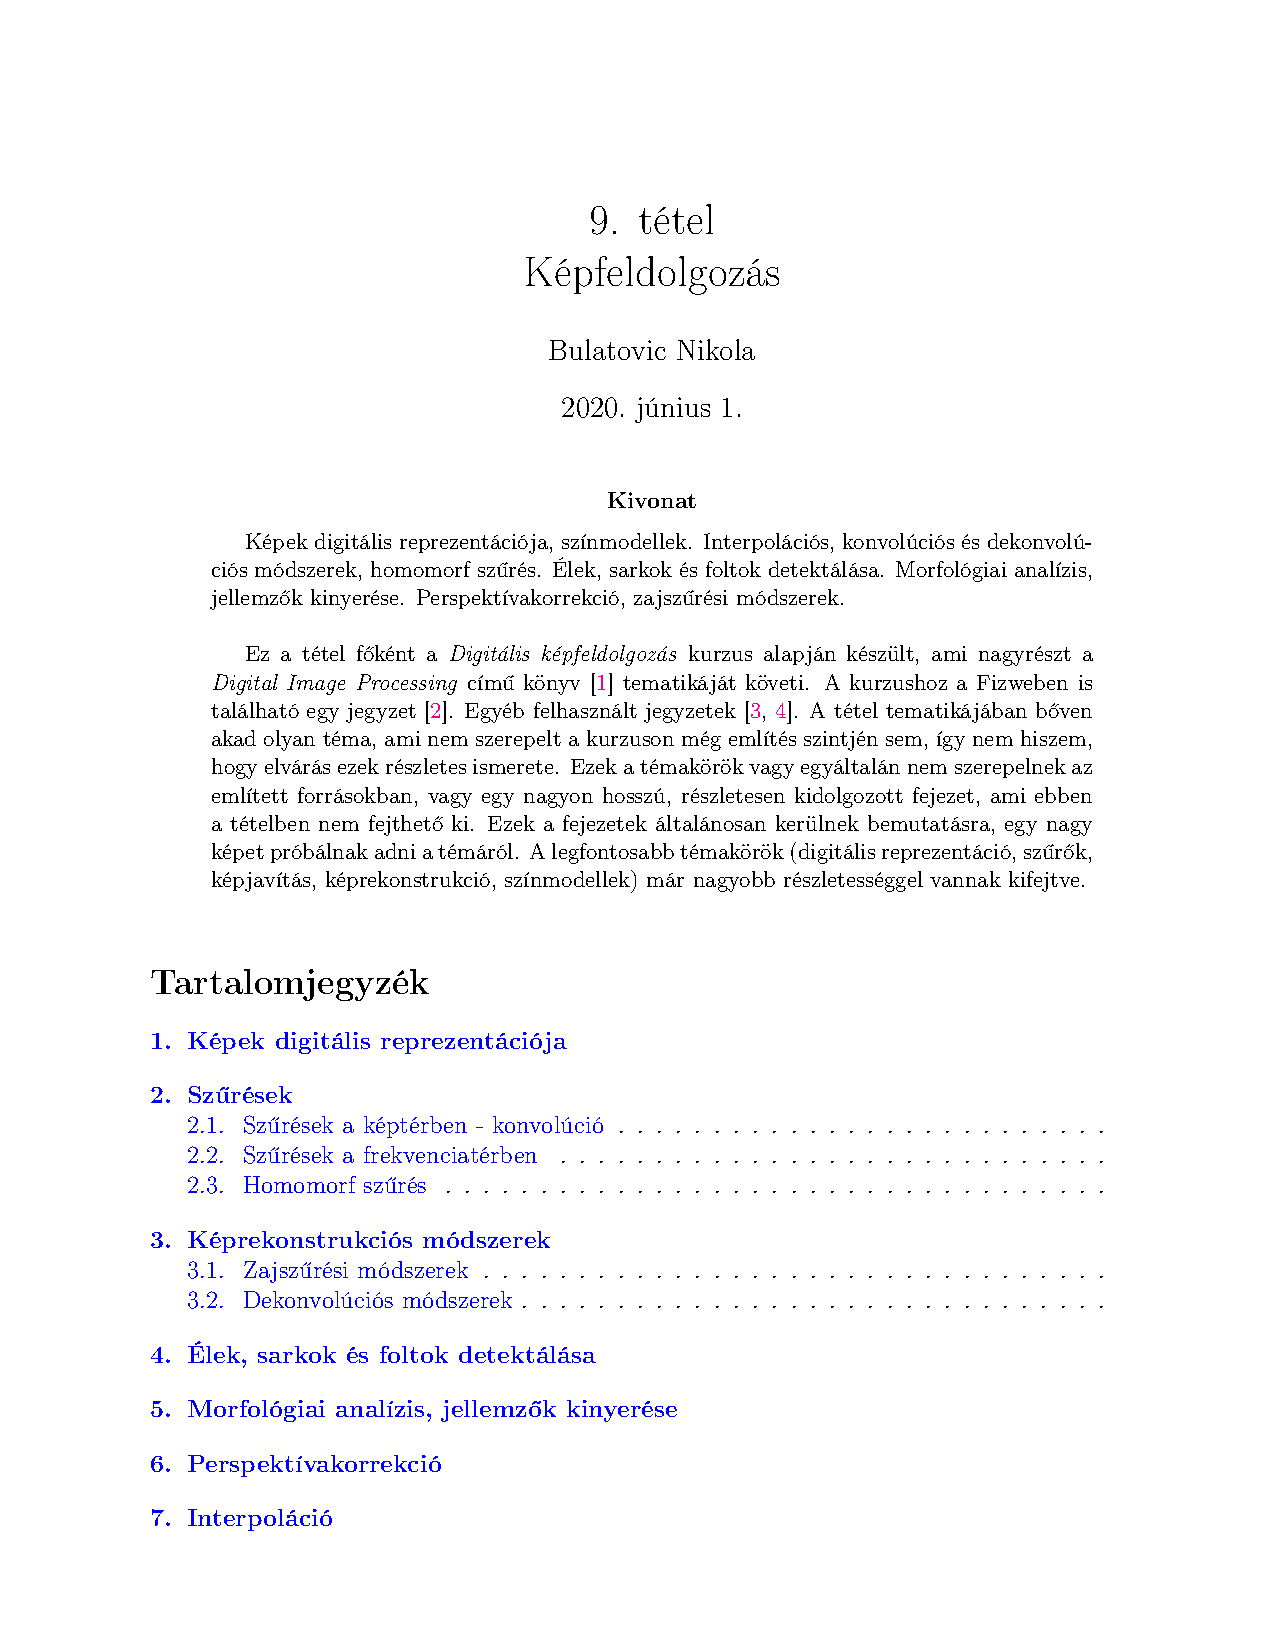
\includepdf[pages=-,addtotoc={
    1,section,1,\textbf{Képfeldolgozás – Képek digitális reprezentációja, színmodellek. Interpolációs, konvolúciós és dekonvolúciós módszerek, homomorf szűrés. Élek, sarkok és foltok detektálása. Morfológiai analízis, jellemzők kinyerése. Perspektívakorrekció, zajszűrési módszerek.},p1}, pagecommand={\thispagestyle{plain}}]{../009/9.pdf}

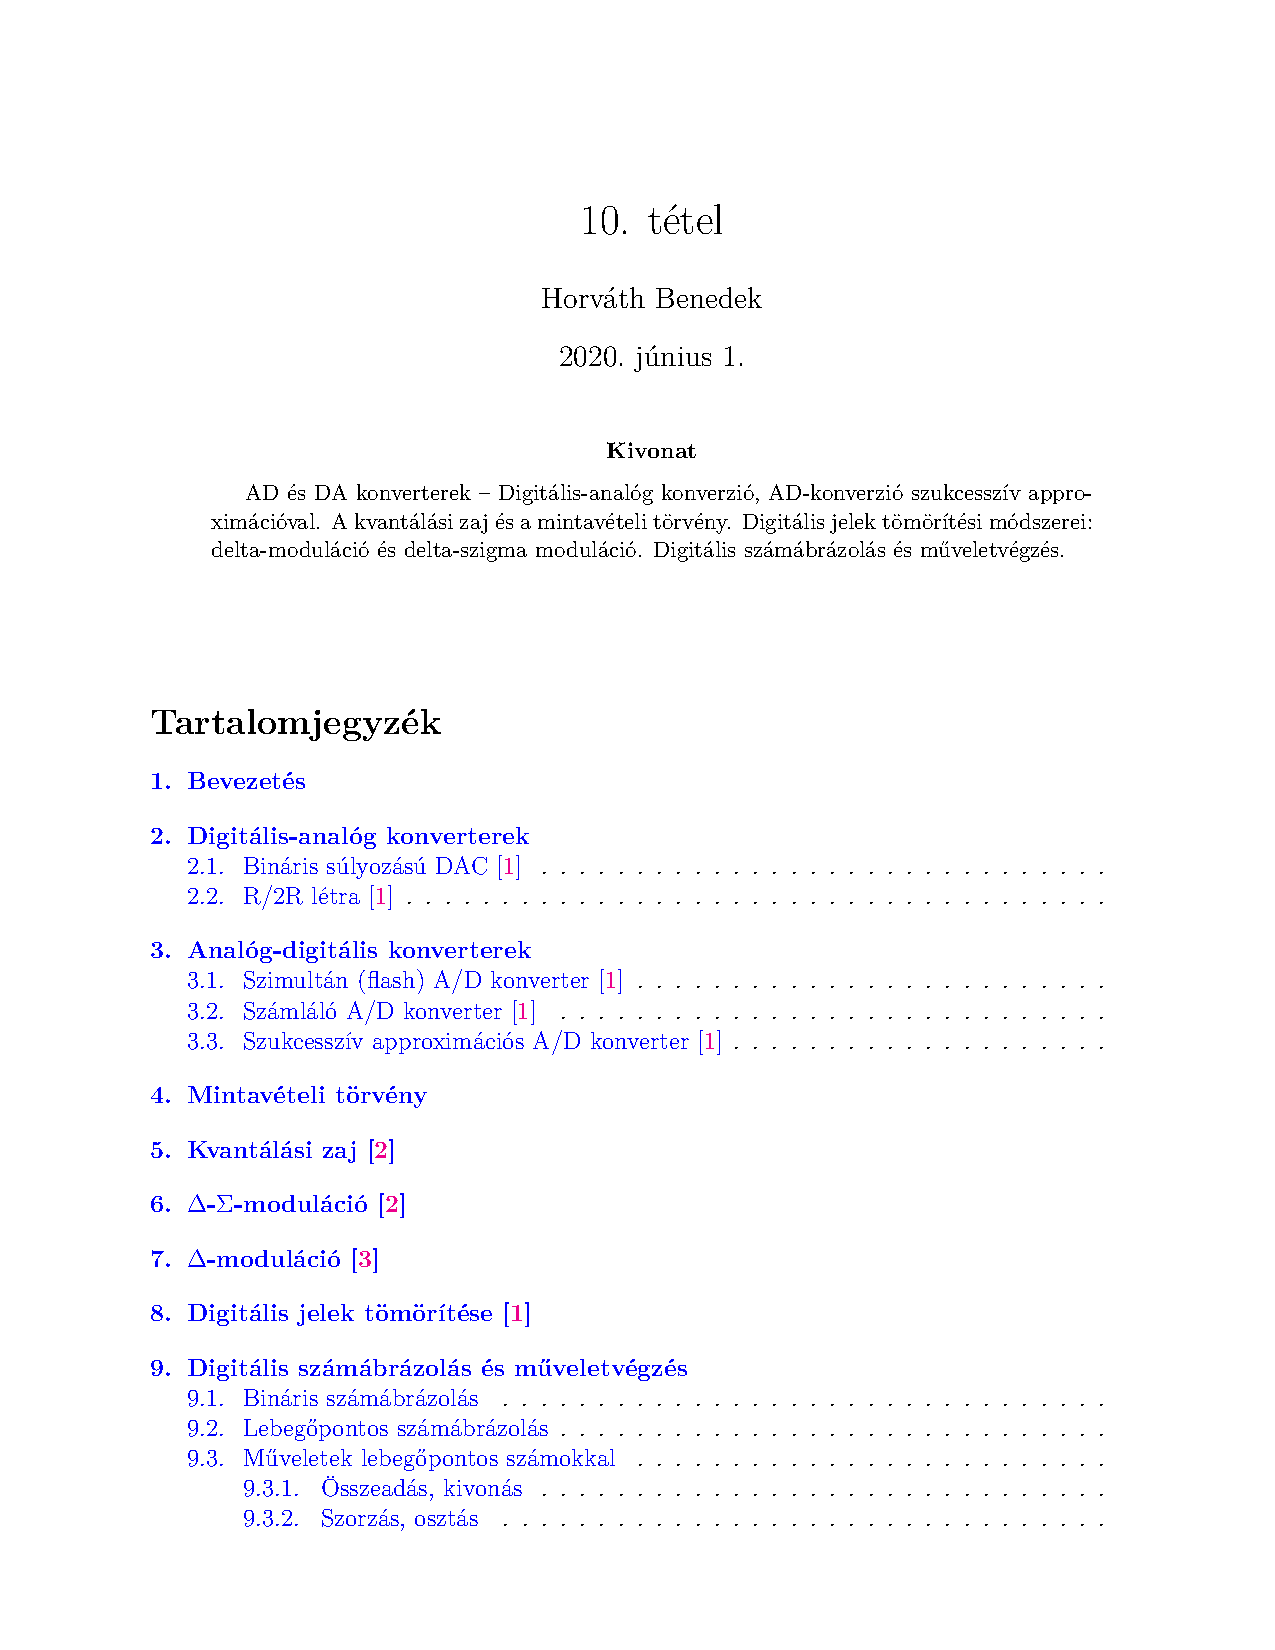
\includepdf[pages=-,addtotoc={
    1,section,1,\textbf{AD és DA konverterek – Digitális-analóg konverzió, AD-konverzió szukcesszív approximációval. A kvantálási zaj és a mintavételi törvény. Digitális jelek tömörítési módszerei: delta-moduláció és delta-szigma moduláció. Digitális számábrázolás és műveletvégzés.},p1}, pagecommand={\thispagestyle{plain}}]{../010/10.pdf}

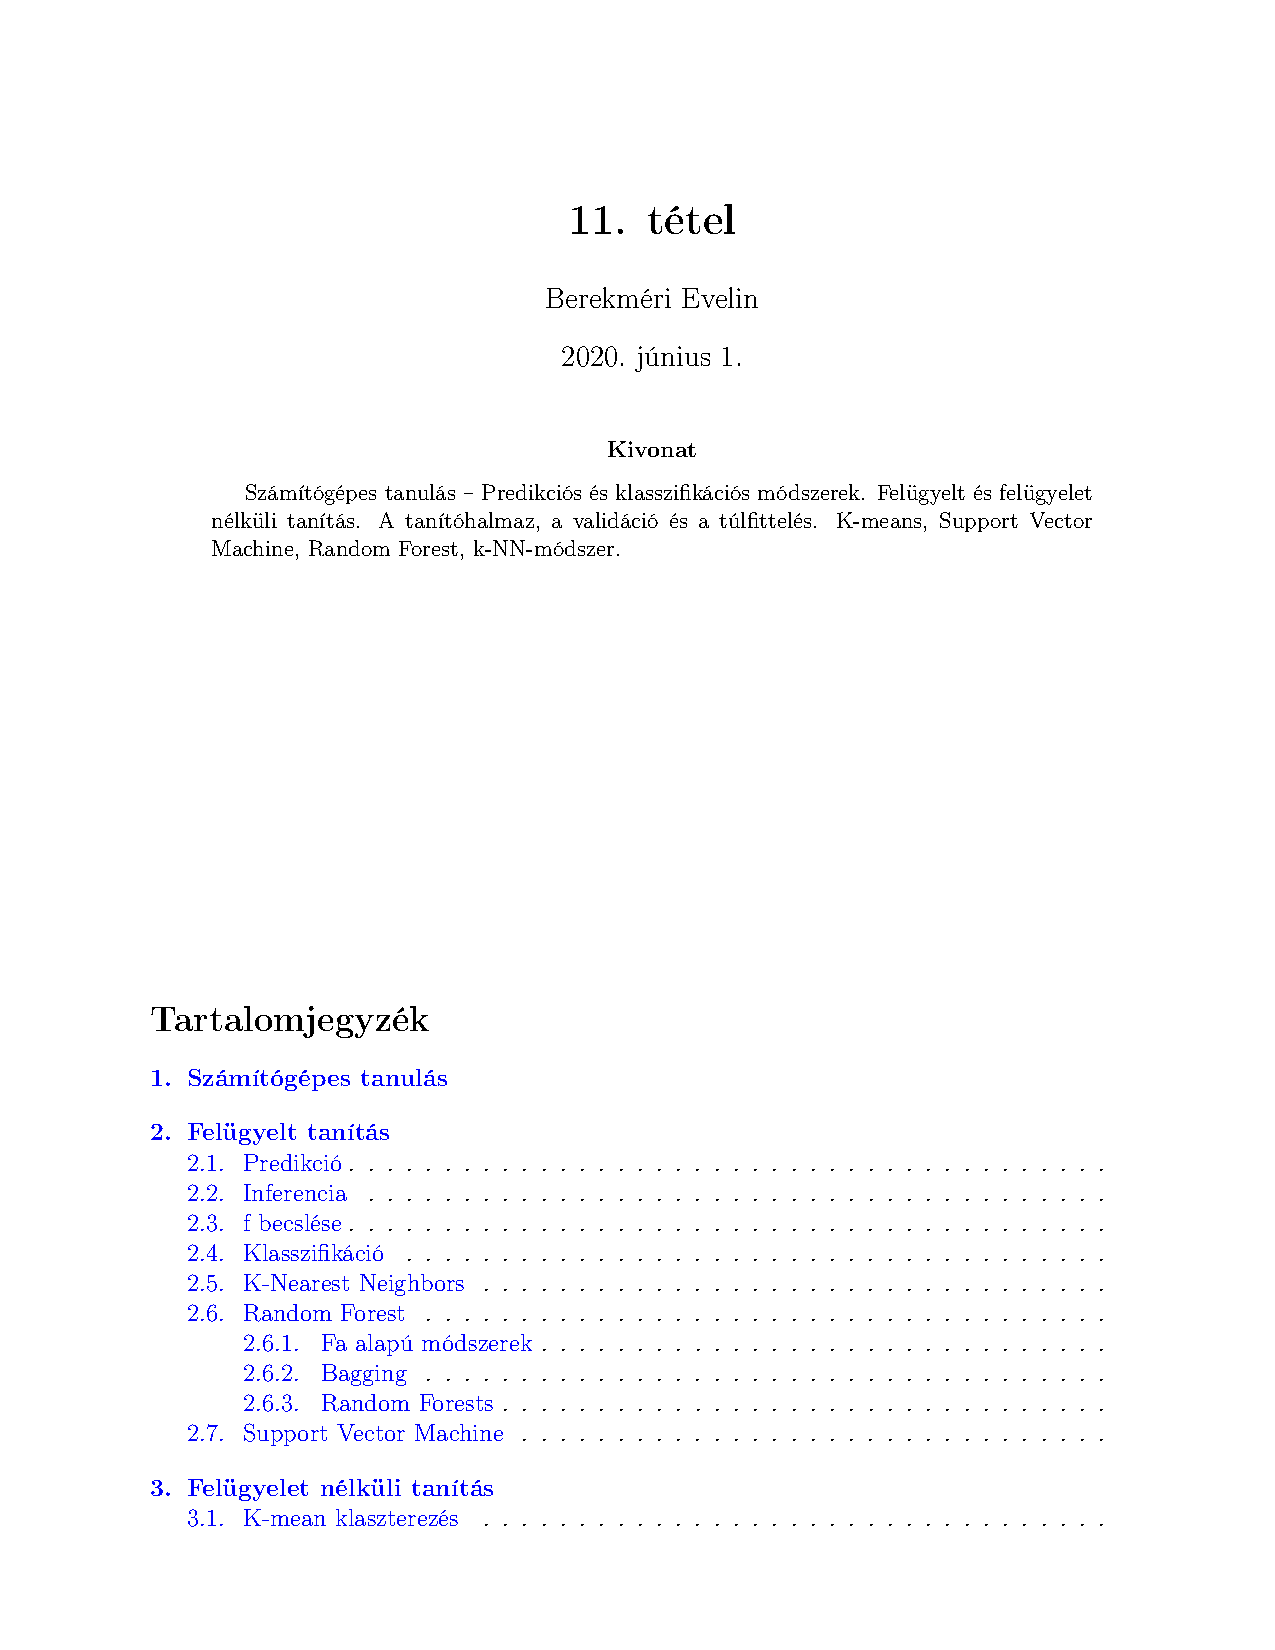
\includepdf[pages=-,addtotoc={
    1,section,1,\textbf{Számítógépes tanulás – Predikciós és klasszifikációs módszerek. Felügyelt és felügyelet nélküli tanítás. A tanítóhalmaz, a validáció és a túlfittelés. K-means, Support Vector Machine, Random Forest, k-NN-módszer. },p1}, pagecommand={\thispagestyle{plain}}]{../011/11.pdf}

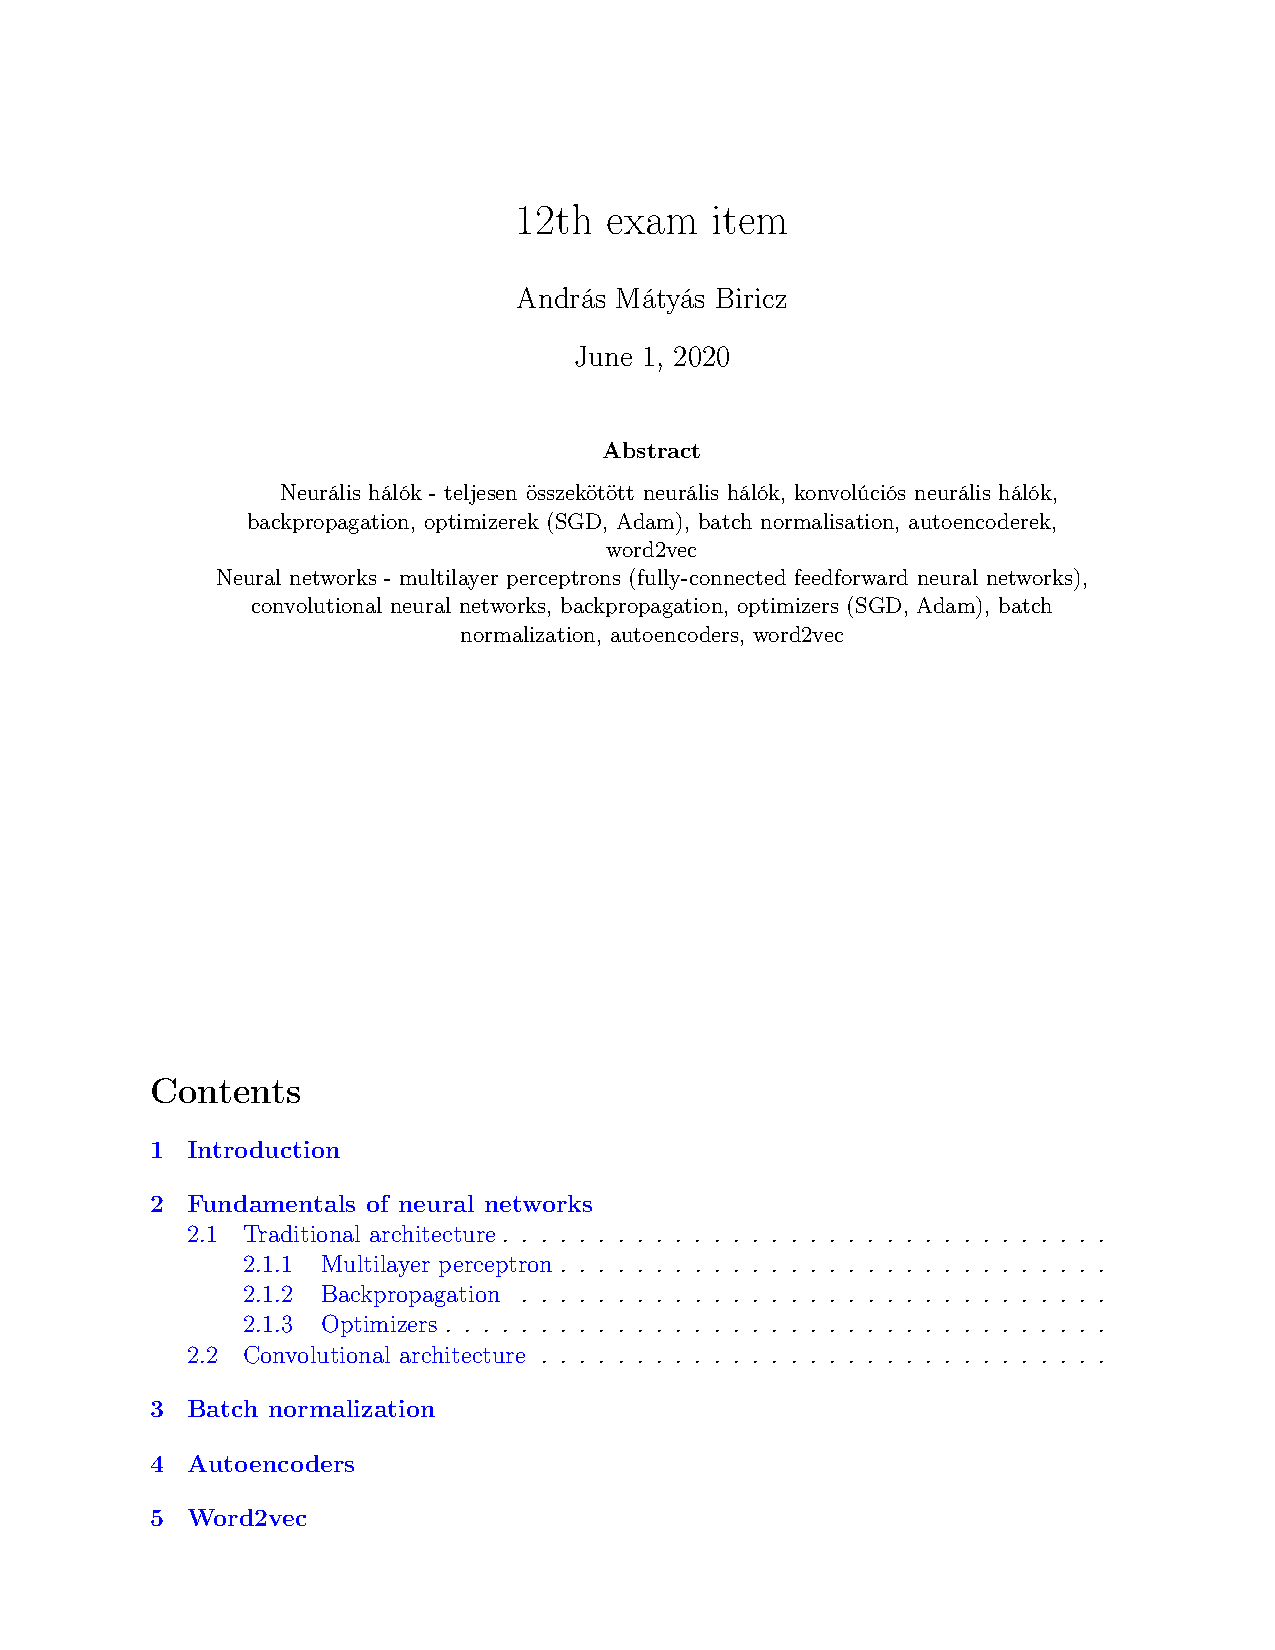
\includepdf[pages=-,addtotoc={
    1,section,1,\textbf{Neurális hálók - teljesen összekötött neurális hálók, konvolúciós neurális hálók, backpropagation, optimizerek (SGD, Adam), batch normalisation, autoencoderek, word2vec},p1}, pagecommand={\thispagestyle{plain}}]{../012/12.pdf}

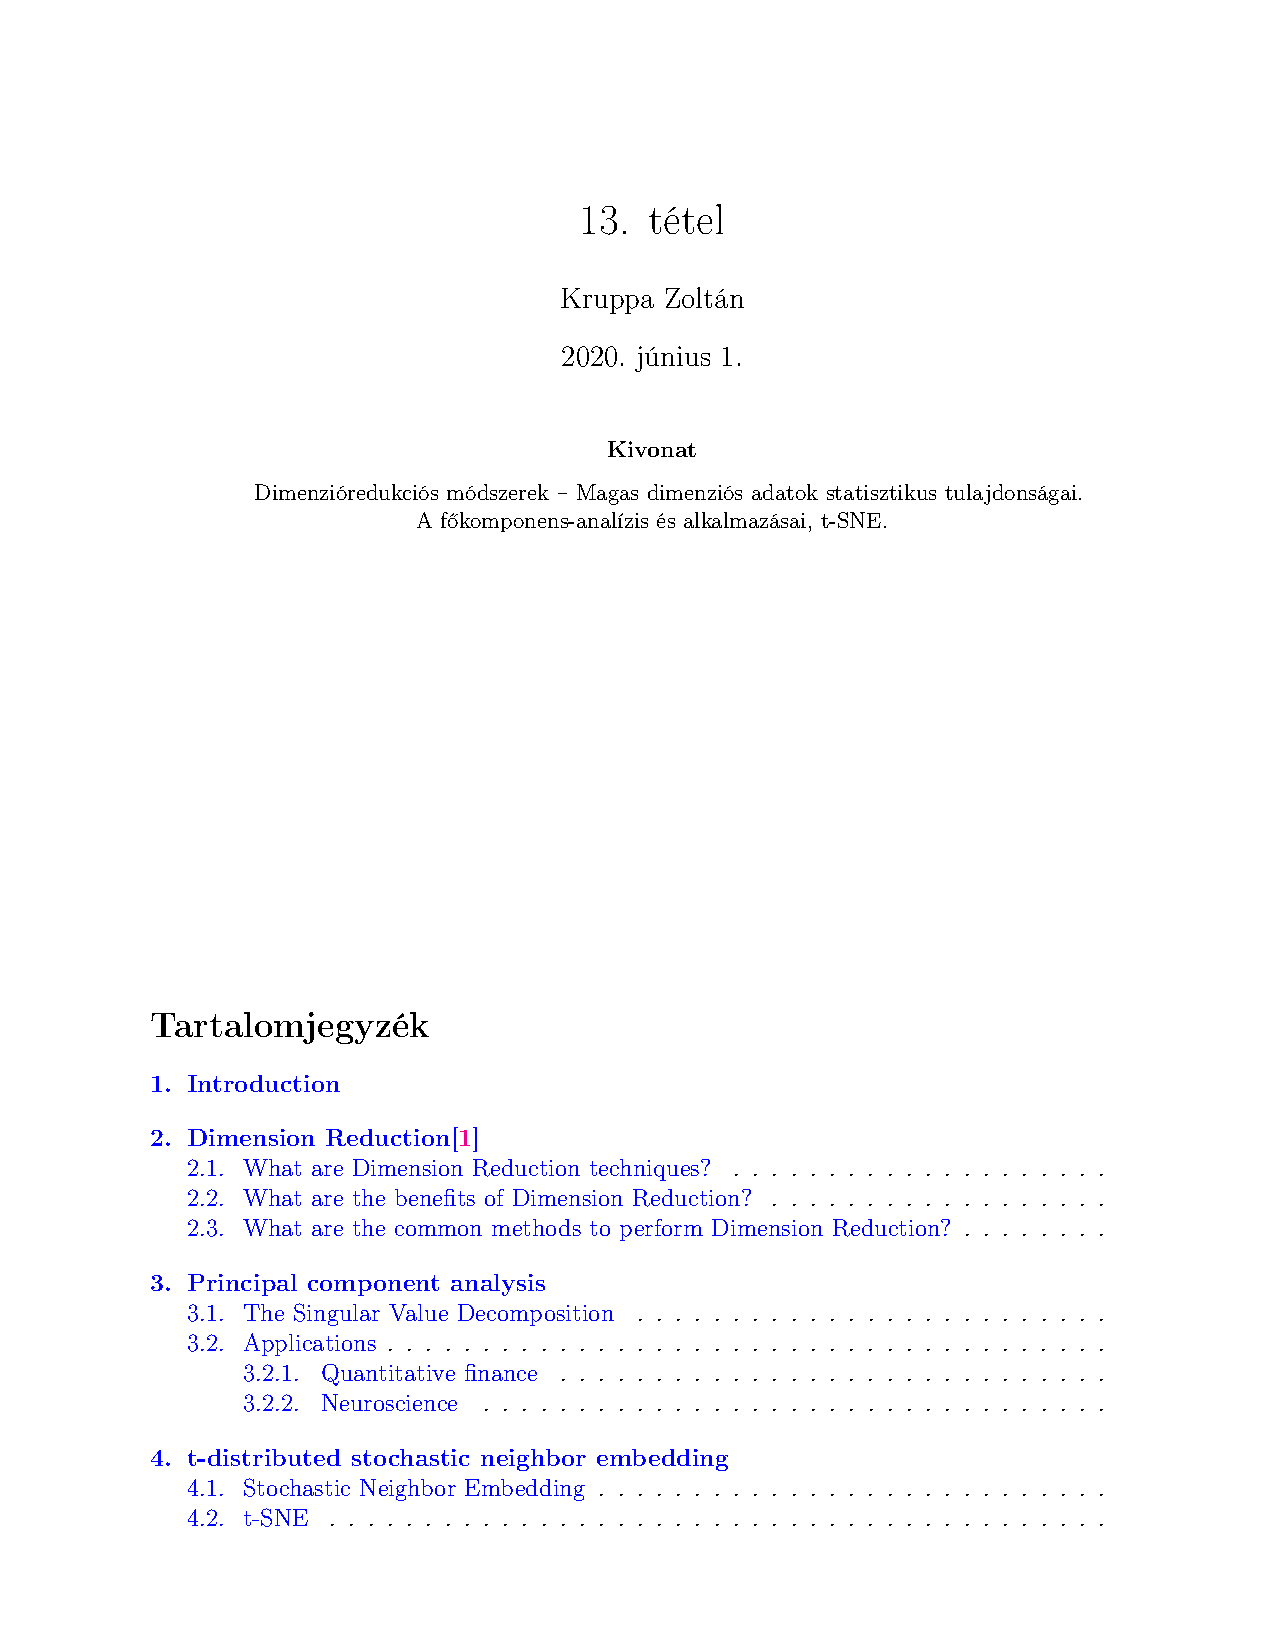
\includepdf[pages=-,addtotoc={
    1,section,1,\textbf{Dimenzióredukciós módszerek – Magas dimenziós adatok statisztikus tulajdonságai. A főkomponens-analízis és alkalmazásai, t-SNE.},p1}, pagecommand={\thispagestyle{plain}}]{../013/13.pdf}

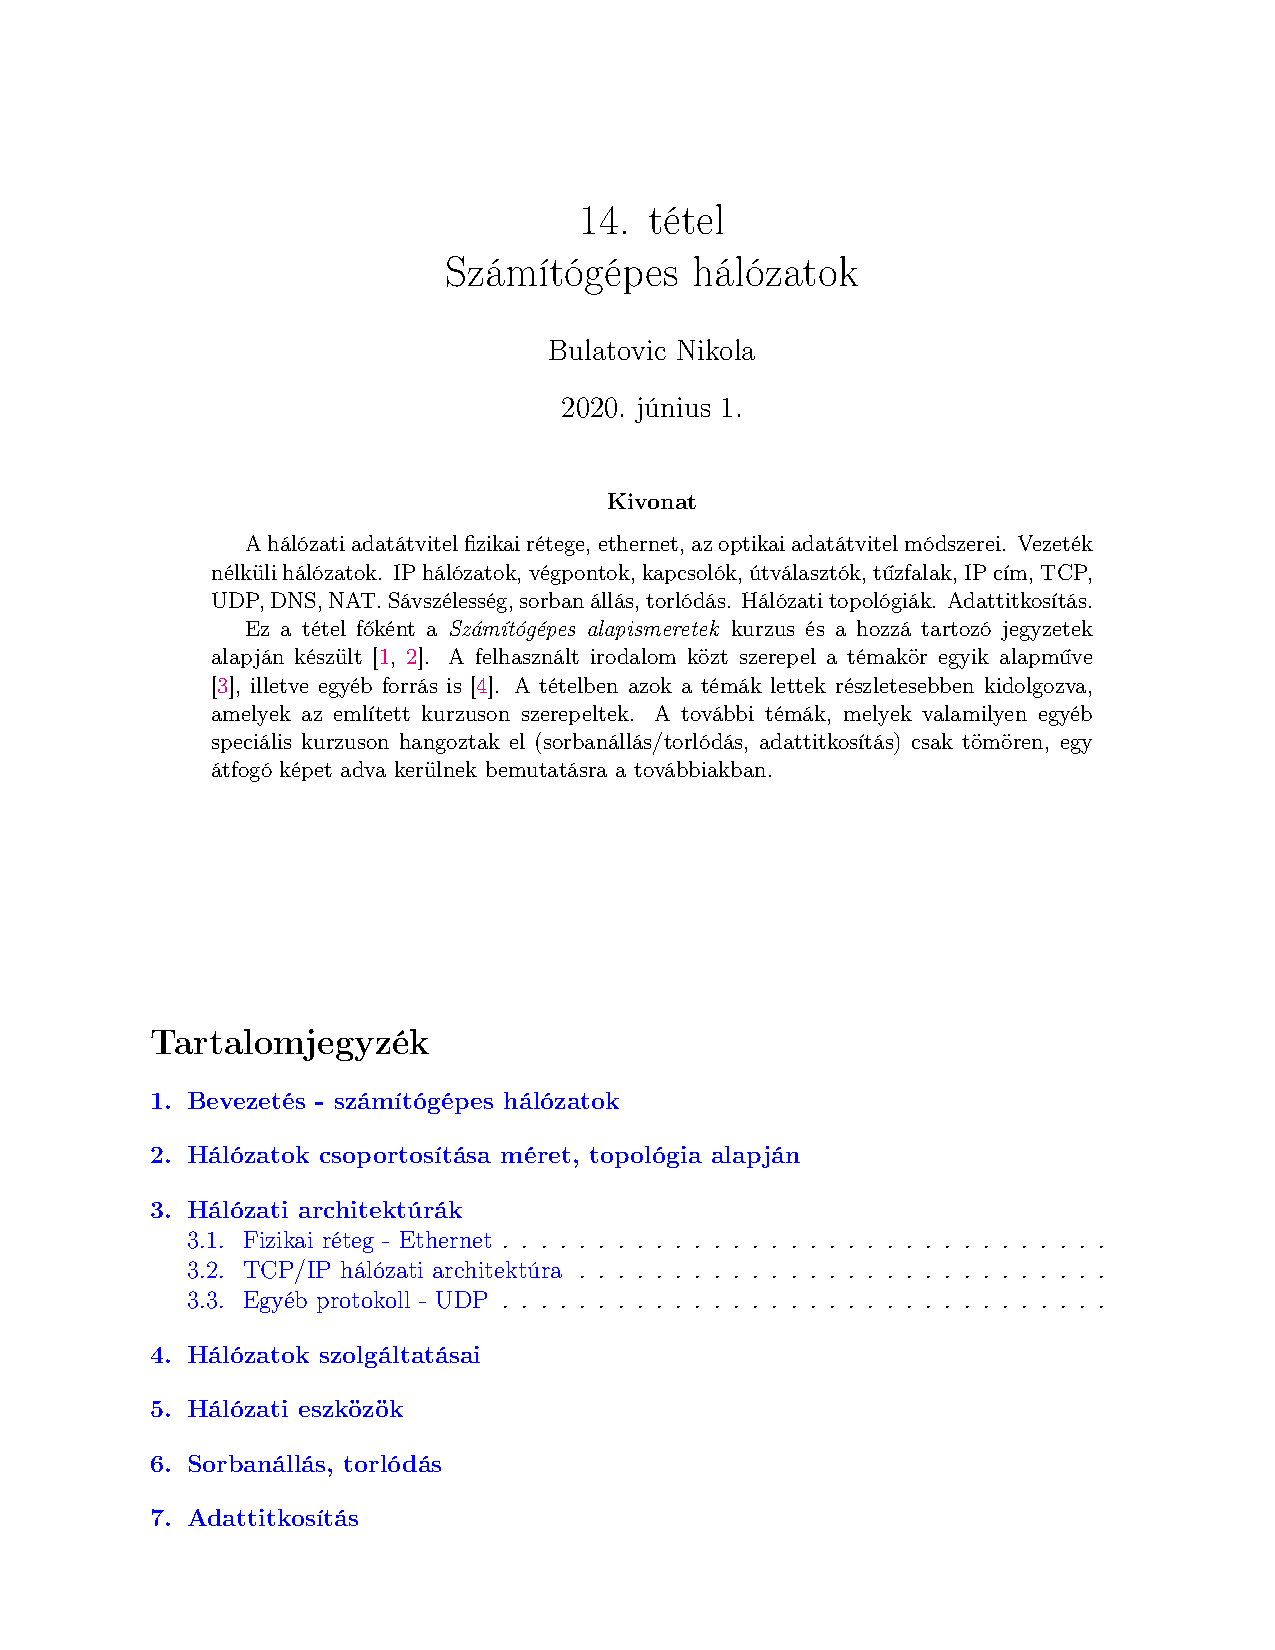
\includepdf[pages=-,addtotoc={
    1,section,1,\textbf{Számítógépes hálózatok – A hálózati adatátvitel fizikai rétege, ethernet, az optikai adatátvitel módszerei. Vezeték nélküli hálózatok. IP hálózatok, végpontok, kapcsolók, útválasztók, tűzfalak, IP cím, TCP, UDP, DNS, NAT. Sávszélesség, sorban állás, torlódás. Hálózati topológiák. Adattitkosítás.},p1}, pagecommand={\thispagestyle{plain}}]{../014/14.pdf}

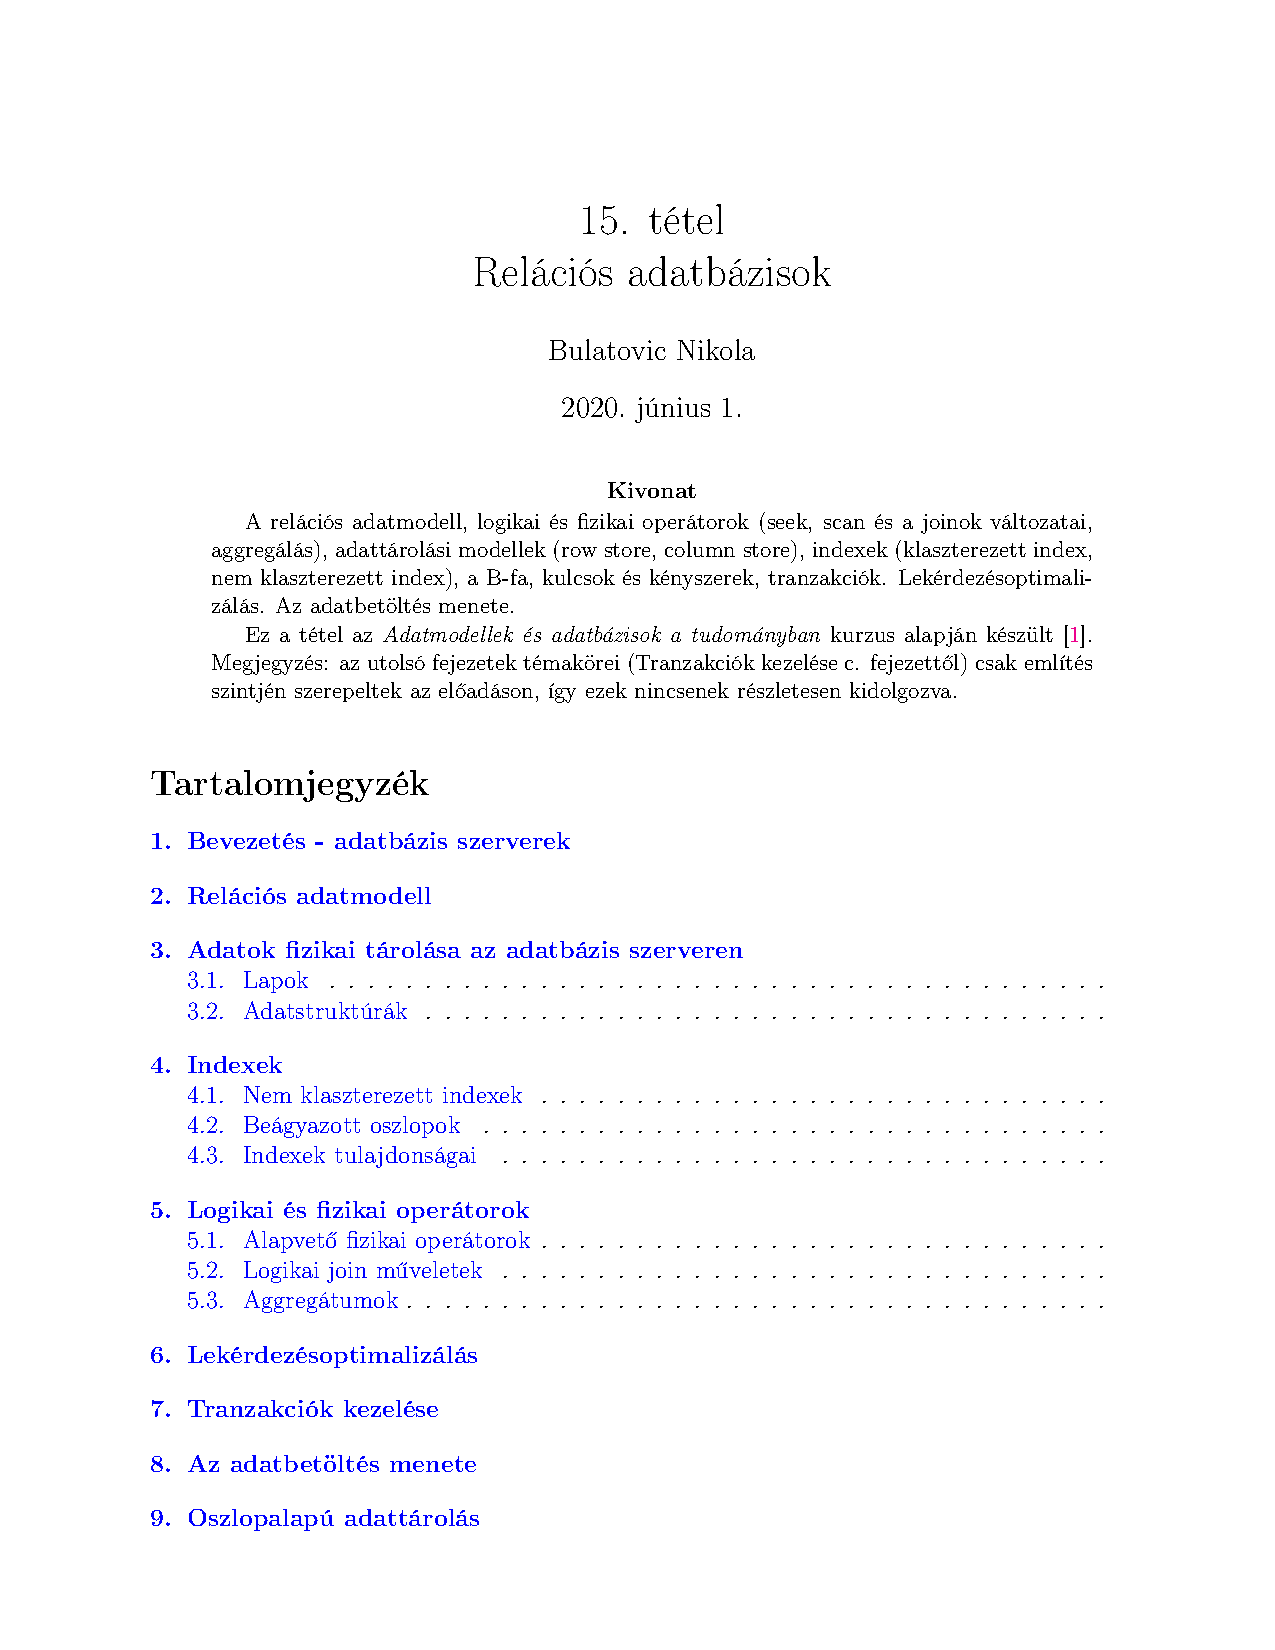
\includepdf[pages=-,addtotoc={
    1,section,1,\textbf{Relációs adatbázisok – a relációs adatmodell, logikai és fizikai operátorok (seek, scan és a joinok változatai, aggregálás), adattárolási modellek (row store, column store), indexek (klaszterezett index, nem klaszterezett index), a B-fa, kulcsok és kényszerek, tranzakciók. Lekérdezésoptimalizálás. Az adatbetöltés menete.},p1}, pagecommand={\thispagestyle{plain}}]{../015/15.pdf}

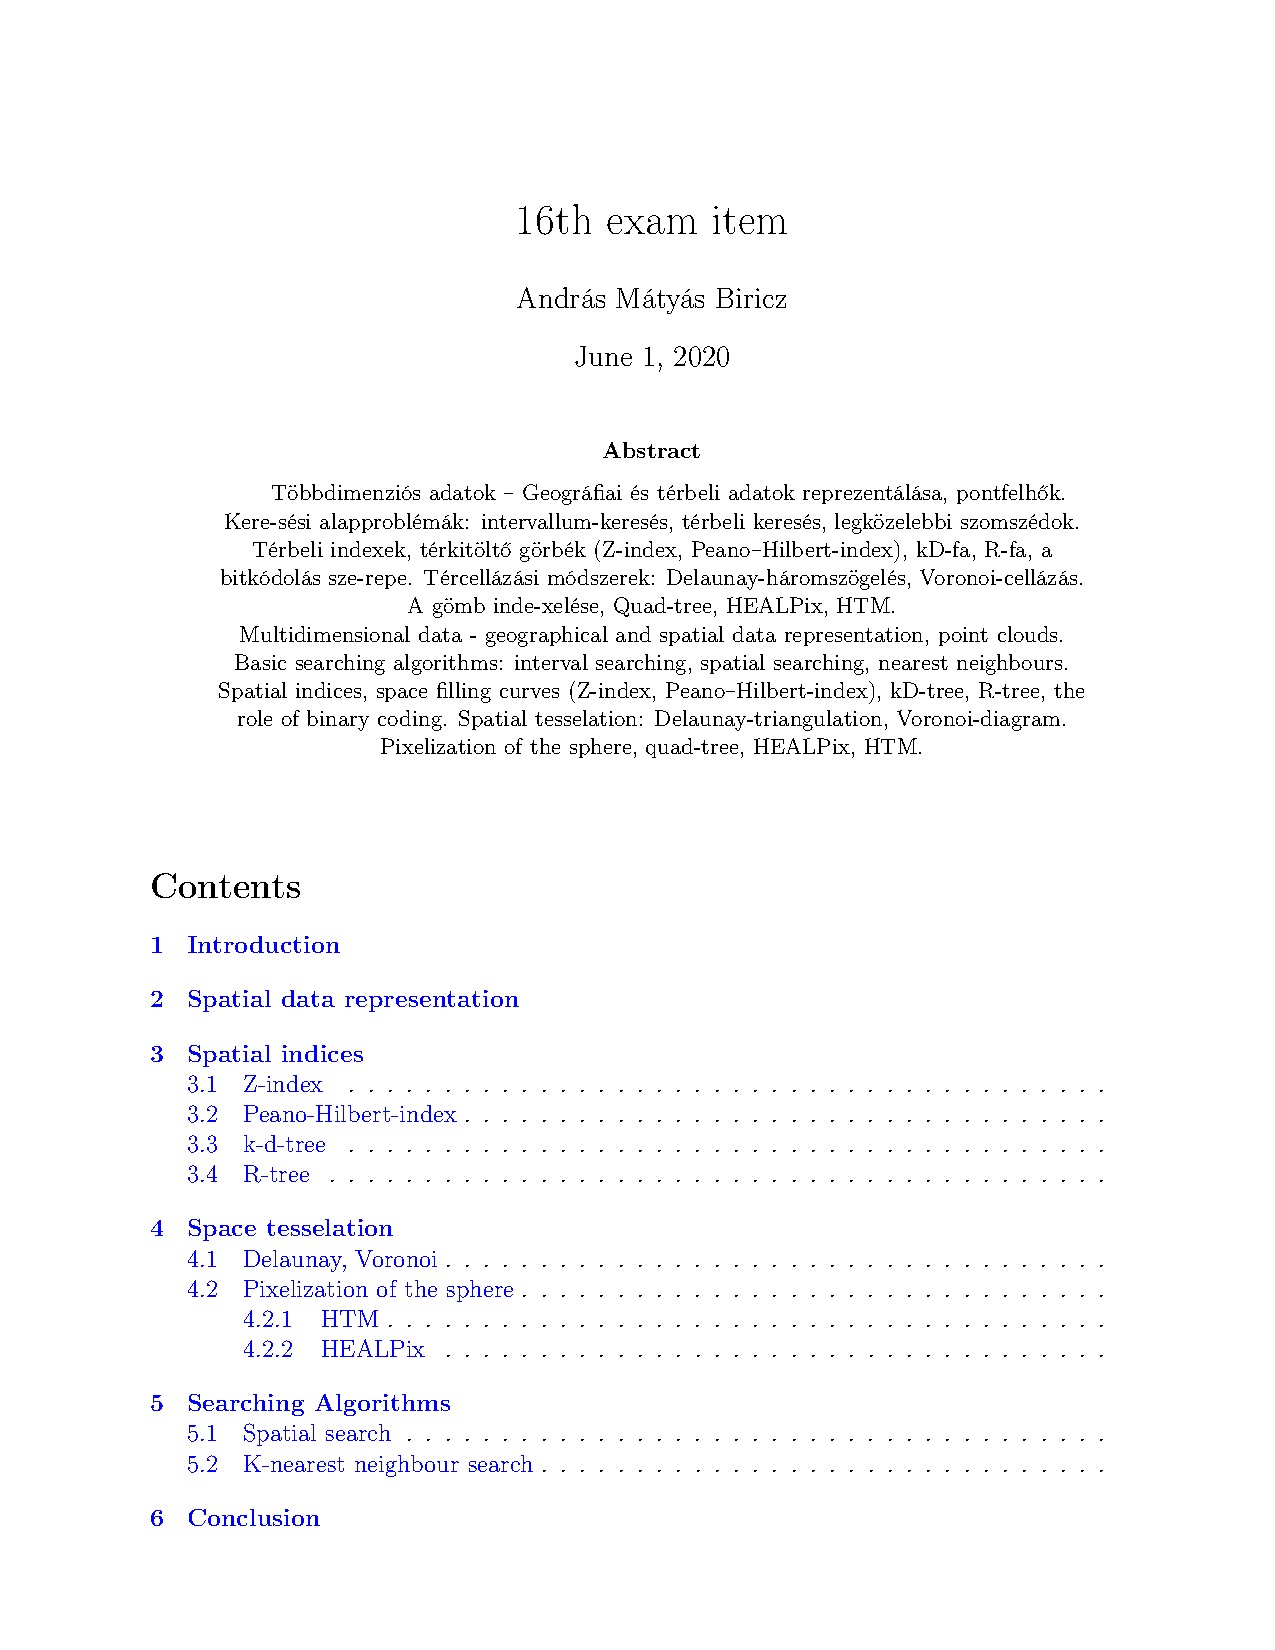
\includepdf[pages=-,addtotoc={
    1,section,1,\textbf{Többdimenziós adatok – Geográfiai és térbeli adatok reprezentálása, pontfelhők. Keresési alapproblémák: intervallum-keresés, térbeli keresés, legközelebbi szomszédok. Térbeli indexek, térkitöltő görbék (Z-index, Peano–Hilbert-index), kD-fa, R-fa, a bitkódolás szerepe. Tércellázási módszerek: Delaunay-háromszögelés, Voronoi-cellázás. A gömb indexelése, Quad-tree, HEALPix, HTM.},p1}, pagecommand={\thispagestyle{plain}}]{../016/16.pdf}

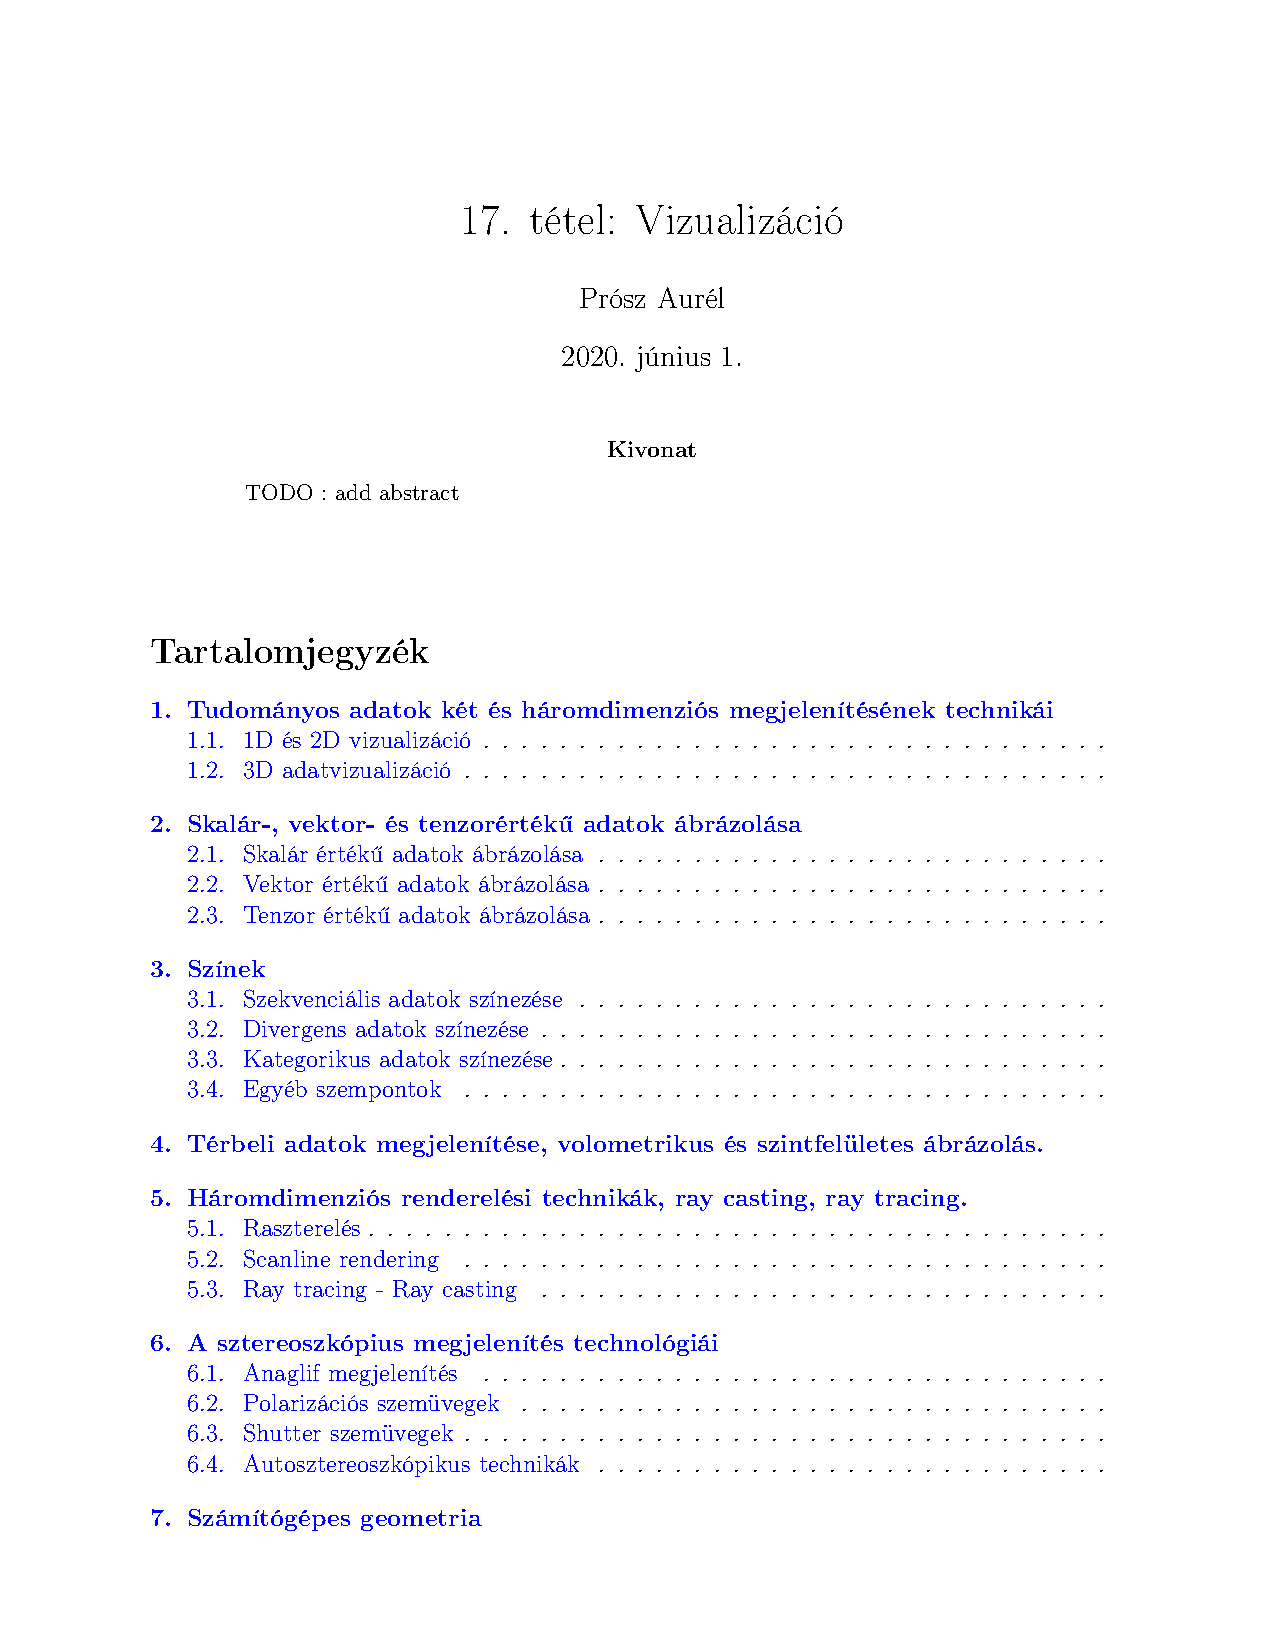
\includepdf[pages=-,addtotoc={
    1,section,1,\textbf{Vizualizáció – Tudományos adatok két és háromdimenziós megjelenítésének technikái, skalár-, vektor- és tenzorértékű adatok ábrázolása. Színek. Térbeli adatok megjelenítése, volometrikus és szintfelületes ábrázolás. Háromdimenziós renderelési technikák, ray casting, ray tracing. A sztereoszkópius megjelenítés technológiái. Számítógépes geometria.},p1}, pagecommand={\thispagestyle{plain}}]{../017/17.pdf}

\end{document}